%&preformat-disser
\RequirePackage[l2tabu,orthodox]{nag} % Раскомментировав, можно в логе получать рекомендации относительно правильного использования пакетов и предупреждения об устаревших и нерекомендуемых пакетах
% Формат А4, 14pt (ГОСТ Р 7.0.11-2011, 5.3.6)
\documentclass[a4paper,14pt,oneside,openany]{memoir}

%%%%%%%%%%%%%%%%%%%%%%%%%%%%%%%%%%%%%%%%%%%%%%%%%%%%%%
%%%% Файл упрощённых настроек шаблона диссертации %%%%
%%%%%%%%%%%%%%%%%%%%%%%%%%%%%%%%%%%%%%%%%%%%%%%%%%%%%%

%%% Инициализирование переменных, не трогать!  %%%
\newcounter{intvl}
\newcounter{otstup}
\newcounter{contnumeq}
\newcounter{contnumfig}
\newcounter{contnumtab}
\newcounter{pgnum}
\newcounter{chapstyle}
\newcounter{headingdelim}
\newcounter{headingalign}
\newcounter{headingsize}
%%%%%%%%%%%%%%%%%%%%%%%%%%%%%%%%%%%%%%%%%%%%%%%%%%%%%%

%%% Область упрощённого управления оформлением %%%

%% Интервал между заголовками и между заголовком и текстом %%
% Заголовки отделяют от текста сверху и снизу
% тремя интервалами (ГОСТ Р 7.0.11-2011, 5.3.5)
\setcounter{intvl}{3}               % Коэффициент кратности к размеру шрифта

%% Отступы у заголовков в тексте %%
\setcounter{otstup}{0}              % 0 --- без отступа; 1 --- абзацный отступ

%% Нумерация формул, таблиц и рисунков %%
% Нумерация формул
\setcounter{contnumeq}{0}   % 0 --- пораздельно (во введении подряд,
                            %       без номера раздела);
                            % 1 --- сквозная нумерация по всей диссертации
% Нумерация рисунков
\setcounter{contnumfig}{0}  % 0 --- пораздельно (во введении подряд,
                            %       без номера раздела);
                            % 1 --- сквозная нумерация по всей диссертации
% Нумерация таблиц
\setcounter{contnumtab}{1}  % 0 --- пораздельно (во введении подряд,
                            %       без номера раздела);
                            % 1 --- сквозная нумерация по всей диссертации

%% Оглавление %%
\setcounter{pgnum}{1}       % 0 --- номера страниц никак не обозначены;
                            % 1 --- Стр. над номерами страниц (дважды
                            %       компилировать после изменения настройки)
\settocdepth{subsection}    % до какого уровня подразделов выносить в оглавление
\setsecnumdepth{subsection} % до какого уровня нумеровать подразделы


%% Текст и форматирование заголовков %%
\setcounter{chapstyle}{0}     % 0 --- разделы только под номером;
                              % 1 --- разделы с названием "Глава" перед номером
\setcounter{headingdelim}{1}  % 0 --- номер отделен пропуском в 1em или \quad;
                              % 1 --- номера разделов и приложений отделены
                              %       точкой с пробелом, подразделы пропуском
                              %       без точки;
                              % 2 --- номера разделов, подразделов и приложений
                              %       отделены точкой с пробелом.

%% Выравнивание заголовков в тексте %%
\setcounter{headingalign}{0}  % 0 --- по центру;
                              % 1 --- по левому краю

%% Размеры заголовков в тексте %%
\setcounter{headingsize}{0}   % 0 --- по ГОСТ, все всегда 14 пт;
                              % 1 --- пропорционально изменяющийся размер
                              %       в зависимости от базового шрифта

%% Подпись таблиц %%

% Смещение строк подписи после первой строки
\newcommand{\tabindent}{0cm}

% Тип форматирования заголовка таблицы:
% plain --- название и текст в одной строке
% split --- название и текст в разных строках
\newcommand{\tabformat}{plain}

%%% Настройки форматирования таблицы `plain`

% Выравнивание по центру подписи, состоящей из одной строки:
% true  --- выравнивать
% false --- не выравнивать
\newcommand{\tabsinglecenter}{false}

% Выравнивание подписи таблиц:
% justified   --- выравнивать как обычный текст («по ширине»)
% centering   --- выравнивать по центру
% centerlast  --- выравнивать по центру только последнюю строку
% centerfirst --- выравнивать по центру только первую строку (не рекомендуется)
% raggedleft  --- выравнивать по правому краю
% raggedright --- выравнивать по левому краю
\newcommand{\tabjust}{justified}

% Разделитель записи «Таблица #» и названия таблицы
\newcommand{\tablabelsep}{~\cyrdash\ }

%%% Настройки форматирования таблицы `split`

% Положение названия таблицы:
% \centering   --- выравнивать по центру
% \raggedleft  --- выравнивать по правому краю
% \raggedright --- выравнивать по левому краю
\newcommand{\splitformatlabel}{\raggedleft}

% Положение текста подписи:
% \centering   --- выравнивать по центру
% \raggedleft  --- выравнивать по правому краю
% \raggedright --- выравнивать по левому краю
\newcommand{\splitformattext}{\raggedright}

%% Подпись рисунков %%
%Разделитель записи «Рисунок #» и названия рисунка
\newcommand{\figlabelsep}{~\cyrdash\ }  % (ГОСТ 2.105, 4.3.1)
                                        % "--- здесь не работает

%%% Цвета гиперссылок %%%
% Latex color definitions: http://latexcolor.com/
\definecolor{linkcolor}{rgb}{0.9,0,0}
\definecolor{citecolor}{rgb}{0,0.6,0}
\definecolor{urlcolor}{rgb}{0,0,1}
%\definecolor{linkcolor}{rgb}{0,0,0} %black
%\definecolor{citecolor}{rgb}{0,0,0} %black
%\definecolor{urlcolor}{rgb}{0,0,0} %black
            % общие настройки шаблона
%%% Проверка используемого TeX-движка %%%
\newif\ifxetexorluatex   % определяем новый условный оператор (http://tex.stackexchange.com/a/47579)
\ifxetex
    \xetexorluatextrue
\else
    \ifluatex
        \xetexorluatextrue
    \else
        \xetexorluatexfalse
    \fi
\fi

\newif\ifsynopsis           % Условие, проверяющее, что документ --- автореферат

\usepackage{etoolbox}[2015/08/02]   % Для продвинутой проверки разных условий
\providebool{presentation}

\usepackage{comment}    % Позволяет убирать блоки текста (добавляет
                        % окружение comment и команду \excludecomment)

%%% Поля и разметка страницы %%%
\usepackage{pdflscape}  % Для включения альбомных страниц
\usepackage{geometry}   % Для последующего задания полей

%%% Математические пакеты %%%
\usepackage{amsthm,amsmath,amscd}   % Математические дополнения от AMS
\usepackage{amsfonts,amssymb}       % Математические дополнения от AMS
\usepackage{mathtools}              % Добавляет окружение multlined
\usepackage{xfrac}                  % Красивые дроби
\usepackage{commath}
\usepackage[
    locale = DE,
    list-separator       = {;\,},
    list-final-separator = {;\,},
    list-pair-separator  = {;\,},
    list-units           = single,
    range-units          = single,
    range-phrase={\text{\ensuremath{-}}},
    % quotient-mode        = fraction, % красивые дроби могут не соответствовать ГОСТ
    fraction-function    = \sfrac,
    separate-uncertainty,
    ]{siunitx}                      % Размерности SI
\sisetup{inter-unit-product = \ensuremath{{}\cdot{}}}

% Кириллица в нумерации subequations
% Для правильной работы требуется выполнение сразу после загрузки пакетов
\patchcmd{\subequations}{\def\theequation{\theparentequation\alph{equation}}}
{\def\theequation{\theparentequation\asbuk{equation}}}
{\typeout{subequations patched}}{\typeout{subequations not patched}}

%%%% Установки для размера шрифта 14 pt %%%%
%% Формирование переменных и констант для сравнения (один раз для всех подключаемых файлов)%%
%% должно располагаться до вызова пакета fontspec или polyglossia, потому что они сбивают его работу
\newlength{\curtextsize}
\newlength{\bigtextsize}
\setlength{\bigtextsize}{13.9pt}

\makeatletter
%\show\f@size    % неплохо для отслеживания, но вызывает стопорение процесса,
                 % если документ компилируется без команды  -interaction=nonstopmode
\setlength{\curtextsize}{\f@size pt}
\makeatother

%%% Кодировки и шрифты %%%
\ifxetexorluatex
    \ifpresentation
        \providecommand*\autodot{} % quick fix for polyglossia 1.50
    \fi
    \PassOptionsToPackage{no-math}{fontspec}    % https://tex.stackexchange.com/a/26295/104425
    \usepackage{polyglossia}[2014/05/21]        % Поддержка многоязычности
                                        % (fontspec подгружается автоматически)
\else
   %%% Решение проблемы копирования текста в буфер кракозябрами
    \ifnumequal{\value{usealtfont}}{0}{}{
        \input glyphtounicode.tex
        \input glyphtounicode-cmr.tex %from pdfx package
        \pdfgentounicode=1
    }
    \usepackage{cmap}   % Улучшенный поиск русских слов в полученном pdf-файле
    \ifnumequal{\value{usealtfont}}{2}{}{
        \defaulthyphenchar=127  % Если стоит до fontenc, то переносы
                                % не впишутся в выделяемый текст при
                                % копировании его в буфер обмена
    }
    \usepackage{textcomp}
    \usepackage[T1,T2A]{fontenc}                    % Поддержка русских букв
    \ifnumequal{\value{usealtfont}}{1}{% Используется pscyr, при наличии
        \IfFileExists{pscyr.sty}{\usepackage{pscyr}}{}  % Подключение pscyr
    }{}
    \usepackage[utf8]{inputenc}[2014/04/30]         % Кодировка utf8
    \usepackage[english, russian]{babel}[2014/03/24]% Языки: русский, английский
    \makeatletter\AtBeginDocument{\let\@elt\relax}\makeatother % babel 3.40 fix
    \ifnumequal{\value{usealtfont}}{2}{
        % http://dxdy.ru/post1238763.html#p1238763
        \usepackage[scaled=0.914]{XCharter}[2017/12/19] % Подключение русифицированных шрифтов XCharter
        \usepackage[charter, vvarbb, scaled=1.048]{newtxmath}[2017/12/14]
        \ifpresentation
        \else
            \setDisplayskipStretch{-0.078}
        \fi
    }{}
\fi

%%% Оформление абзацев %%%
\ifpresentation
\else
    \indentafterchapter     % Красная строка после заголовков типа chapter
    \usepackage{indentfirst}
\fi

%%% Цвета %%%
\ifpresentation
\else
    \usepackage[dvipsnames, table, hyperref]{xcolor} % Совместимо с tikz
\fi

%%% Таблицы %%%
\usepackage{longtable,ltcaption} % Длинные таблицы
\usepackage{multirow,makecell}   % Улучшенное форматирование таблиц
\usepackage{tabu, tabulary}      % таблицы с автоматически подбирающейся
                                 % шириной столбцов (tabu обязательно
                                 % до hyperref вызывать)
\usepackage{threeparttable}      % автоматический подгон ширины подписи таблицы

%%% Общее форматирование
\usepackage{soulutf8}% Поддержка переносоустойчивых подчёркиваний и зачёркиваний
\usepackage{icomma}  % Запятая в десятичных дробях

%%% Оптимизация расстановки переносов и длины последней строки абзаца
\IfFileExists{impnattypo.sty}{% проверка установленности пакета impnattypo
    \ifluatex
        \ifnumequal{\value{draft}}{1}{% Черновик
            \usepackage[hyphenation, lastparline, nosingleletter, homeoarchy,
            rivers, draft]{impnattypo}
        }{% Чистовик
            \usepackage[hyphenation, lastparline, nosingleletter]{impnattypo}
        }
    \else
        \usepackage[hyphenation, lastparline]{impnattypo}
    \fi
}{}

%% Векторная графика

\usepackage{tikz}                   % Продвинутый пакет векторной графики
\usetikzlibrary{chains}             % Для примера tikz рисунка
\usetikzlibrary{shapes.geometric}   % Для примера tikz рисунка
\usetikzlibrary{shapes.symbols}     % Для примера tikz рисунка
\usetikzlibrary{arrows}             % Для примера tikz рисунка

%%% Гиперссылки %%%
\ifxetexorluatex
    \let\CYRDZE\relax
\fi
\usepackage{hyperref}[2012/11/06]

%%% Изображения %%%
\usepackage{graphicx}[2014/04/25]   % Подключаем пакет работы с графикой
\usepackage{caption}                % Подписи рисунков и таблиц
\usepackage{subcaption}             % Подписи подрисунков и подтаблиц
\usepackage{pdfpages}               % Добавление внешних pdf файлов

%%% Счётчики %%%
\usepackage{aliascnt}
\usepackage[figure,table]{totalcount}   % Счётчик рисунков и таблиц
\usepackage{totcount}   % Пакет создания счётчиков на основе последнего номера
                        % подсчитываемого элемента (может требовать дважды
                        % компилировать документ)
\usepackage{totpages}   % Счётчик страниц, совместимый с hyperref (ссылается
                        % на номер последней страницы). Желательно ставить
                        % последним пакетом в преамбуле

%%% Продвинутое управление групповыми ссылками (пока только формулами) %%%
\ifpresentation
\else
    \usepackage[russian]{cleveref} % cleveref имеет сложности со считыванием
    % языка из babel. Такое решение русификации вывода выбрано вместо
    % определения в documentclass из опасности что-то лишнее передать во все
    % остальные пакеты, включая библиографию.

    % Добавление возможности использования пробелов в \labelcref
    % https://tex.stackexchange.com/a/340502/104425
    \usepackage{kvsetkeys}
    \makeatletter
    \let\org@@cref\@cref
    \renewcommand*{\@cref}[2]{%
        \edef\process@me{%
            \noexpand\org@@cref{#1}{\zap@space#2 \@empty}%
        }\process@me
    }
    \makeatother
\fi

\usepackage{placeins} % для \FloatBarrier

\ifnumequal{\value{draft}}{1}{% Черновик
    \usepackage[firstpage]{draftwatermark}
    \SetWatermarkText{DRAFT}
    \SetWatermarkFontSize{14pt}
    \SetWatermarkScale{15}
    \SetWatermarkAngle{45}
}{}

%%% Цитата, не приводимая в автореферате:
% возможно, актуальна только для biblatex
%\newcommand{\citeinsynopsis}[1]{\ifsynopsis\else ~\cite{#1} \fi}

% если текущий процесс запущен библиотекой tikz-external, то прекомпиляция должна быть включена
\ifdefined\tikzexternalrealjob
    \setcounter{imgprecompile}{1}
\fi

\ifnumequal{\value{imgprecompile}}{1}{% Только если у нас включена предкомпиляция
    \usetikzlibrary{external}   % подключение возможности предкомпиляции
    \tikzexternalize[prefix=images/cache/,optimize command away=\includepdf] % activate! % здесь можно указать отдельную папку для скомпилированных файлов
    \ifxetex
        \tikzset{external/up to date check={diff}}
    \fi
}{}


         % Пакеты общие для диссертации и автореферата
\synopsisfalse                      % Этот документ --- не автореферат
\input{Dissertation/dispackages}    % Пакеты для диссертации
\input{Dissertation/userpackages}   % Пакеты для специфических пользовательских задач

%%%%%%%%%%%%%%%%%%%%%%%%%%%%%%%%%%%%%%%%%%%%%%%%%%%%%%
%%%% Файл упрощённых настроек шаблона диссертации %%%%
%%%%%%%%%%%%%%%%%%%%%%%%%%%%%%%%%%%%%%%%%%%%%%%%%%%%%%

%%% Инициализирование переменных, не трогать!  %%%
\newcounter{intvl}
\newcounter{otstup}
\newcounter{contnumeq}
\newcounter{contnumfig}
\newcounter{contnumtab}
\newcounter{pgnum}
\newcounter{chapstyle}
\newcounter{headingdelim}
\newcounter{headingalign}
\newcounter{headingsize}
%%%%%%%%%%%%%%%%%%%%%%%%%%%%%%%%%%%%%%%%%%%%%%%%%%%%%%

%%% Область упрощённого управления оформлением %%%

%% Интервал между заголовками и между заголовком и текстом %%
% Заголовки отделяют от текста сверху и снизу
% тремя интервалами (ГОСТ Р 7.0.11-2011, 5.3.5)
\setcounter{intvl}{3}               % Коэффициент кратности к размеру шрифта

%% Отступы у заголовков в тексте %%
\setcounter{otstup}{0}              % 0 --- без отступа; 1 --- абзацный отступ

%% Нумерация формул, таблиц и рисунков %%
% Нумерация формул
\setcounter{contnumeq}{0}   % 0 --- пораздельно (во введении подряд,
                            %       без номера раздела);
                            % 1 --- сквозная нумерация по всей диссертации
% Нумерация рисунков
\setcounter{contnumfig}{0}  % 0 --- пораздельно (во введении подряд,
                            %       без номера раздела);
                            % 1 --- сквозная нумерация по всей диссертации
% Нумерация таблиц
\setcounter{contnumtab}{1}  % 0 --- пораздельно (во введении подряд,
                            %       без номера раздела);
                            % 1 --- сквозная нумерация по всей диссертации

%% Оглавление %%
\setcounter{pgnum}{1}       % 0 --- номера страниц никак не обозначены;
                            % 1 --- Стр. над номерами страниц (дважды
                            %       компилировать после изменения настройки)
\settocdepth{subsection}    % до какого уровня подразделов выносить в оглавление
\setsecnumdepth{subsection} % до какого уровня нумеровать подразделы


%% Текст и форматирование заголовков %%
\setcounter{chapstyle}{0}     % 0 --- разделы только под номером;
                              % 1 --- разделы с названием "Глава" перед номером
\setcounter{headingdelim}{1}  % 0 --- номер отделен пропуском в 1em или \quad;
                              % 1 --- номера разделов и приложений отделены
                              %       точкой с пробелом, подразделы пропуском
                              %       без точки;
                              % 2 --- номера разделов, подразделов и приложений
                              %       отделены точкой с пробелом.

%% Выравнивание заголовков в тексте %%
\setcounter{headingalign}{0}  % 0 --- по центру;
                              % 1 --- по левому краю

%% Размеры заголовков в тексте %%
\setcounter{headingsize}{0}   % 0 --- по ГОСТ, все всегда 14 пт;
                              % 1 --- пропорционально изменяющийся размер
                              %       в зависимости от базового шрифта

%% Подпись таблиц %%

% Смещение строк подписи после первой строки
\newcommand{\tabindent}{0cm}

% Тип форматирования заголовка таблицы:
% plain --- название и текст в одной строке
% split --- название и текст в разных строках
\newcommand{\tabformat}{plain}

%%% Настройки форматирования таблицы `plain`

% Выравнивание по центру подписи, состоящей из одной строки:
% true  --- выравнивать
% false --- не выравнивать
\newcommand{\tabsinglecenter}{false}

% Выравнивание подписи таблиц:
% justified   --- выравнивать как обычный текст («по ширине»)
% centering   --- выравнивать по центру
% centerlast  --- выравнивать по центру только последнюю строку
% centerfirst --- выравнивать по центру только первую строку (не рекомендуется)
% raggedleft  --- выравнивать по правому краю
% raggedright --- выравнивать по левому краю
\newcommand{\tabjust}{justified}

% Разделитель записи «Таблица #» и названия таблицы
\newcommand{\tablabelsep}{~\cyrdash\ }

%%% Настройки форматирования таблицы `split`

% Положение названия таблицы:
% \centering   --- выравнивать по центру
% \raggedleft  --- выравнивать по правому краю
% \raggedright --- выравнивать по левому краю
\newcommand{\splitformatlabel}{\raggedleft}

% Положение текста подписи:
% \centering   --- выравнивать по центру
% \raggedleft  --- выравнивать по правому краю
% \raggedright --- выравнивать по левому краю
\newcommand{\splitformattext}{\raggedright}

%% Подпись рисунков %%
%Разделитель записи «Рисунок #» и названия рисунка
\newcommand{\figlabelsep}{~\cyrdash\ }  % (ГОСТ 2.105, 4.3.1)
                                        % "--- здесь не работает

%%% Цвета гиперссылок %%%
% Latex color definitions: http://latexcolor.com/
\definecolor{linkcolor}{rgb}{0.9,0,0}
\definecolor{citecolor}{rgb}{0,0.6,0}
\definecolor{urlcolor}{rgb}{0,0,1}
%\definecolor{linkcolor}{rgb}{0,0,0} %black
%\definecolor{citecolor}{rgb}{0,0,0} %black
%\definecolor{urlcolor}{rgb}{0,0,0} %black
      % Упрощённые настройки шаблона

\input{common/newnames}         % Новые переменные, для всего проекта

%%% Основные сведения %%%
\newcommand{\thesisAuthorLastName}{\fixme{Абдуллин}}
\newcommand{\thesisAuthorOtherNames}{\fixme{Рустам Фаритович}}
\newcommand{\thesisAuthorInitials}{\fixme{Р.\,Ф.}}
\newcommand{\thesisAuthor}             % Диссертация, ФИО автора
{%
    \texorpdfstring{% \texorpdfstring takes two arguments and uses the first for (La)TeX and the second for pdf
        \thesisAuthorLastName~\thesisAuthorOtherNames% так будет отображаться на титульном листе или в тексте, где будет использоваться переменная
    }{%
        \thesisAuthorLastName, \thesisAuthorOtherNames% эта запись для свойств pdf-файла. В таком виде, если pdf будет обработан программами для сбора библиографических сведений, будет правильно представлена фамилия.
    }
}
\newcommand{\thesisAuthorShort}        % Диссертация, ФИО автора инициалами
{\thesisAuthorInitials~\thesisAuthorLastName}
%\newcommand{\thesisUdk}                % Диссертация, УДК
%{\fixme{xxx.xxx}}
\newcommand{\thesisTitle}              % Диссертация, название
{\fixme{Построение матрицы жесткости для слоистой среды в
методе разрывных смещений}}
\newcommand{\thesisSpecialtyNumber}    % Диссертация, специальность, номер
{\fixme{01.04.03}}
\newcommand{\thesisSpecialtyTitle}     % Диссертация, специальность, название (название взято с сайта ВАК для примера)
{\fixme{Механика и математическое моделирование}}
%% \newcommand{\thesisSpecialtyTwoNumber} % Диссертация, вторая специальность, номер
%% {\fixme{XX.XX.XX}}
%% \newcommand{\thesisSpecialtyTwoTitle}  % Диссертация, вторая специальность, название
%% {\fixme{Теория и~методика физического воспитания, спортивной тренировки,
%% оздоровительной и~адаптивной физической культуры}}
\newcommand{\thesisDegree}             % Диссертация, ученая степень
{\fixme{кандидата физико-математических наук}}
\newcommand{\thesisDegreeShort}        % Диссертация, ученая степень, краткая запись
{\fixme{канд. физ.-мат. наук}}
\newcommand{\thesisCity}               % Диссертация, город написания диссертации
{\fixme{Новосибирск}}
\newcommand{\thesisYear}               % Диссертация, год написания диссертации
{\the\year}
\newcommand{\thesisOrganization}       % Диссертация, организация
{\fixme{''Новосибирский национальный исследовательский государственный университет'', НГУ}}
\newcommand{\thesisOrganizationShort}  % Диссертация, краткое название организации для доклада
{\fixme{НГУ}}

\newcommand{\thesisInOrganization}     % Диссертация, организация в предложном падеже: Работа выполнена в ...
{\fixme{учреждении с~длинным длинным длинным длинным названием, в~котором
выполнялась данная диссертационная работа}}

%% \newcommand{\supervisorDead}{}           % Рисовать рамку вокруг фамилии
\newcommand{\supervisorFio}              % Научный руководитель, ФИО
{\fixme{Головин Сергей Валерьевич}}
\newcommand{\supervisorRegalia}          % Научный руководитель, регалии
{\fixme{д-р физ.-мат.~наук, проф.~РАН}}
\newcommand{\supervisorFioShort}         % Научный руководитель, ФИО
{\fixme{С.\,В.~Головин}}
\newcommand{\supervisorRegaliaShort}     % Научный руководитель, регалии
{\fixme{д-р~физ.-мат.~наук, проф.~РАН}}

%% \newcommand{\supervisorTwoDead}{}        % Рисовать рамку вокруг фамилии
%% \newcommand{\supervisorTwoFio}           % Второй научный руководитель, ФИО
%% {\fixme{Фамилия Имя Отчество}}
%% \newcommand{\supervisorTwoRegalia}       % Второй научный руководитель, регалии
%% {\fixme{уч. степень, уч. звание}}
%% \newcommand{\supervisorTwoFioShort}      % Второй научный руководитель, ФИО
%% {\fixme{И.\,О.~Фамилия}}
%% \newcommand{\supervisorTwoRegaliaShort}  % Второй научный руководитель, регалии
%% {\fixme{уч.~ст.,~уч.~зв.}}

\newcommand{\opponentOneFio}           % Оппонент 1, ФИО
{\fixme{Фамилия Имя Отчество}}
\newcommand{\opponentOneRegalia}       % Оппонент 1, регалии
{\fixme{доктор физико-математических наук, профессор}}
\newcommand{\opponentOneJobPlace}      % Оппонент 1, место работы
{\fixme{Не очень длинное название для места работы}}
\newcommand{\opponentOneJobPost}       % Оппонент 1, должность
{\fixme{старший научный сотрудник}}

\newcommand{\opponentTwoFio}           % Оппонент 2, ФИО
{\fixme{Фамилия Имя Отчество}}
\newcommand{\opponentTwoRegalia}       % Оппонент 2, регалии
{\fixme{кандидат физико-математических наук}}
\newcommand{\opponentTwoJobPlace}      % Оппонент 2, место работы
{\fixme{Основное место работы c длинным длинным длинным длинным названием}}
\newcommand{\opponentTwoJobPost}       % Оппонент 2, должность
{\fixme{старший научный сотрудник}}

%% \newcommand{\opponentThreeFio}         % Оппонент 3, ФИО
%% {\fixme{Фамилия Имя Отчество}}
%% \newcommand{\opponentThreeRegalia}     % Оппонент 3, регалии
%% {\fixme{кандидат физико-математических наук}}
%% \newcommand{\opponentThreeJobPlace}    % Оппонент 3, место работы
%% {\fixme{Основное место работы c длинным длинным длинным длинным названием}}
%% \newcommand{\opponentThreeJobPost}     % Оппонент 3, должность
%% {\fixme{старший научный сотрудник}}

\newcommand{\leadingOrganizationTitle} % Ведущая организация, дополнительные строки. Удалить, чтобы не отображать в автореферате
{\fixme{Федеральное государственное бюджетное образовательное учреждение высшего
профессионального образования с~длинным длинным длинным длинным названием}}

\newcommand{\defenseDate}              % Защита, дата
{\fixme{DD mmmmmmmm YYYY~г.~в~XX часов}}
\newcommand{\defenseCouncilNumber}     % Защита, номер диссертационного совета
{\fixme{Д\,123.456.78}}
\newcommand{\defenseCouncilTitle}      % Защита, учреждение диссертационного совета
{\fixme{Название учреждения}}
\newcommand{\defenseCouncilAddress}    % Защита, адрес учреждение диссертационного совета
{\fixme{Адрес}}
\newcommand{\defenseCouncilPhone}      % Телефон для справок
{\fixme{+7~(0000)~00-00-00}}

\newcommand{\defenseSecretaryFio}      % Секретарь диссертационного совета, ФИО
{\fixme{Фамилия Имя Отчество}}
\newcommand{\defenseSecretaryRegalia}  % Секретарь диссертационного совета, регалии
{\fixme{д-р~физ.-мат. наук}}            % Для сокращений есть ГОСТы, например: ГОСТ Р 7.0.12-2011 + http://base.garant.ru/179724/#block_30000

\newcommand{\synopsisLibrary}          % Автореферат, название библиотеки
{\fixme{Название библиотеки}}
\newcommand{\synopsisDate}             % Автореферат, дата рассылки
{\fixme{DD mmmmmmmm}\the\year~года}

% To avoid conflict with beamer class use \providecommand
\providecommand{\keywords}%            % Ключевые слова для метаданных PDF диссертации и автореферата
{}
             % Основные сведения
\input{common/fonts}            % Определение шрифтов (частичное)
%%% Шаблон %%%
\DeclareRobustCommand{\fixme}{\textcolor{black}}  % решаем проблему превращения
                                % названия цвета в результате \MakeUppercase,
                                % http://tex.stackexchange.com/a/187930,
                                % \DeclareRobustCommand protects \fixme
                                % from expanding inside \MakeUppercase
\AtBeginDocument{%
    \setlength{\parindent}{2.5em}                   % Абзацный отступ. Должен быть одинаковым по всему тексту и равен пяти знакам (ГОСТ Р 7.0.11-2011, 5.3.7).
}

%%% Таблицы %%%
\DeclareCaptionLabelSeparator{tabsep}{\tablabelsep} % нумерация таблиц
\DeclareCaptionFormat{split}{\splitformatlabel#1\par\splitformattext#3}

\captionsetup[table]{
        format=\tabformat,                % формат подписи (plain|hang)
        font=normal,                      % нормальные размер, цвет, стиль шрифта
        skip=.0pt,                        % отбивка под подписью
        parskip=.0pt,                     % отбивка между параграфами подписи
        position=above,                   % положение подписи
        justification=\tabjust,           % центровка
        indent=\tabindent,                % смещение строк после первой
        labelsep=tabsep,                  % разделитель
        singlelinecheck=\tabsinglecenter, % не выравнивать по центру, если умещается в одну строку
}

%%% Рисунки %%%
\DeclareCaptionLabelSeparator{figsep}{\figlabelsep} % нумерация рисунков

\captionsetup[figure]{
        format=plain,                     % формат подписи (plain|hang)
        font=normal,                      % нормальные размер, цвет, стиль шрифта
        skip=.0pt,                        % отбивка под подписью
        parskip=.0pt,                     % отбивка между параграфами подписи
        position=below,                   % положение подписи
        singlelinecheck=true,             % выравнивание по центру, если умещается в одну строку
        justification=centerlast,         % центровка
        labelsep=figsep,                  % разделитель
}

%%% Подписи подрисунков %%%
\DeclareCaptionSubType{figure}
\renewcommand\thesubfigure{\asbuk{subfigure}} % нумерация подрисунков
\ifsynopsis
\DeclareCaptionFont{norm}{\fontsize{10pt}{11pt}\selectfont}
\newcommand{\subfigureskip}{2.pt}
\else
\DeclareCaptionFont{norm}{\fontsize{14pt}{16pt}\selectfont}
\newcommand{\subfigureskip}{0.pt}
\fi

\captionsetup[subfloat]{
        labelfont=norm,                 % нормальный размер подписей подрисунков
        textfont=norm,                  % нормальный размер подписей подрисунков
        labelsep=space,                 % разделитель
        labelformat=brace,              % одна скобка справа от номера
        justification=centering,        % центровка
        singlelinecheck=true,           % выравнивание по центру, если умещается в одну строку
        skip=\subfigureskip,            % отбивка над подписью
        parskip=.0pt,                   % отбивка между параграфами подписи
        position=below,                 % положение подписи
}

%%% Настройки ссылок на рисунки, таблицы и др. %%%
% команды \cref...format отвечают за форматирование при помощи команды \cref
% команды \labelcref...format отвечают за форматирование при помощи команды \labelcref

\ifpresentation
\else
    \crefdefaultlabelformat{#2#1#3}

    % Уравнение
    \crefformat{equation}{(#2#1#3)} % одиночная ссылка с приставкой
    \labelcrefformat{equation}{(#2#1#3)} % одиночная ссылка без приставки
    \crefrangeformat{equation}{(#3#1#4) \cyrdash~(#5#2#6)} % диапазон ссылок с приставкой
    \labelcrefrangeformat{equation}{(#3#1#4) \cyrdash~(#5#2#6)} % диапазон ссылок без приставки
    \crefmultiformat{equation}{(#2#1#3)}{ и~(#2#1#3)}{, (#2#1#3)}{ и~(#2#1#3)} % перечисление ссылок с приставкой
    \labelcrefmultiformat{equation}{(#2#1#3)}{ и~(#2#1#3)}{, (#2#1#3)}{ и~(#2#1#3)} % перечисление без приставки

    % Подуравнение
    \crefformat{subequation}{(#2#1#3)} % одиночная ссылка с приставкой
    \labelcrefformat{subequation}{(#2#1#3)} % одиночная ссылка без приставки
    \crefrangeformat{subequation}{(#3#1#4) \cyrdash~(#5#2#6)} % диапазон ссылок с приставкой
    \labelcrefrangeformat{subequation}{(#3#1#4) \cyrdash~(#5#2#6)} % диапазон ссылок без приставки
    \crefmultiformat{subequation}{(#2#1#3)}{ и~(#2#1#3)}{, (#2#1#3)}{ и~(#2#1#3)} % перечисление ссылок с приставкой
    \labelcrefmultiformat{subequation}{(#2#1#3)}{ и~(#2#1#3)}{, (#2#1#3)}{ и~(#2#1#3)} % перечисление без приставки

    % Глава
    \crefformat{chapter}{#2#1#3} % одиночная ссылка с приставкой
    \labelcrefformat{chapter}{#2#1#3} % одиночная ссылка без приставки
    \crefrangeformat{chapter}{#3#1#4 \cyrdash~#5#2#6} % диапазон ссылок с приставкой
    \labelcrefrangeformat{chapter}{#3#1#4 \cyrdash~#5#2#6} % диапазон ссылок без приставки
    \crefmultiformat{chapter}{#2#1#3}{ и~#2#1#3}{, #2#1#3}{ и~#2#1#3} % перечисление ссылок с приставкой
    \labelcrefmultiformat{chapter}{#2#1#3}{ и~#2#1#3}{, #2#1#3}{ и~#2#1#3} % перечисление без приставки

    % Параграф
    \crefformat{section}{#2#1#3} % одиночная ссылка с приставкой
    \labelcrefformat{section}{#2#1#3} % одиночная ссылка без приставки
    \crefrangeformat{section}{#3#1#4 \cyrdash~#5#2#6} % диапазон ссылок с приставкой
    \labelcrefrangeformat{section}{#3#1#4 \cyrdash~#5#2#6} % диапазон ссылок без приставки
    \crefmultiformat{section}{#2#1#3}{ и~#2#1#3}{, #2#1#3}{ и~#2#1#3} % перечисление ссылок с приставкой
    \labelcrefmultiformat{section}{#2#1#3}{ и~#2#1#3}{, #2#1#3}{ и~#2#1#3} % перечисление без приставки

    % Приложение
    \crefformat{appendix}{#2#1#3} % одиночная ссылка с приставкой
    \labelcrefformat{appendix}{#2#1#3} % одиночная ссылка без приставки
    \crefrangeformat{appendix}{#3#1#4 \cyrdash~#5#2#6} % диапазон ссылок с приставкой
    \labelcrefrangeformat{appendix}{#3#1#4 \cyrdash~#5#2#6} % диапазон ссылок без приставки
    \crefmultiformat{appendix}{#2#1#3}{ и~#2#1#3}{, #2#1#3}{ и~#2#1#3} % перечисление ссылок с приставкой
    \labelcrefmultiformat{appendix}{#2#1#3}{ и~#2#1#3}{, #2#1#3}{ и~#2#1#3} % перечисление без приставки

    % Рисунок
    \crefformat{figure}{#2#1#3} % одиночная ссылка с приставкой
    \labelcrefformat{figure}{#2#1#3} % одиночная ссылка без приставки
    \crefrangeformat{figure}{#3#1#4 \cyrdash~#5#2#6} % диапазон ссылок с приставкой
    \labelcrefrangeformat{figure}{#3#1#4 \cyrdash~#5#2#6} % диапазон ссылок без приставки
    \crefmultiformat{figure}{#2#1#3}{ и~#2#1#3}{, #2#1#3}{ и~#2#1#3} % перечисление ссылок с приставкой
    \labelcrefmultiformat{figure}{#2#1#3}{ и~#2#1#3}{, #2#1#3}{ и~#2#1#3} % перечисление без приставки

    % Таблица
    \crefformat{table}{#2#1#3} % одиночная ссылка с приставкой
    \labelcrefformat{table}{#2#1#3} % одиночная ссылка без приставки
    \crefrangeformat{table}{#3#1#4 \cyrdash~#5#2#6} % диапазон ссылок с приставкой
    \labelcrefrangeformat{table}{#3#1#4 \cyrdash~#5#2#6} % диапазон ссылок без приставки
    \crefmultiformat{table}{#2#1#3}{ и~#2#1#3}{, #2#1#3}{ и~#2#1#3} % перечисление ссылок с приставкой
    \labelcrefmultiformat{table}{#2#1#3}{ и~#2#1#3}{, #2#1#3}{ и~#2#1#3} % перечисление без приставки

    % Листинг
    \crefformat{lstlisting}{#2#1#3} % одиночная ссылка с приставкой
    \labelcrefformat{lstlisting}{#2#1#3} % одиночная ссылка без приставки
    \crefrangeformat{lstlisting}{#3#1#4 \cyrdash~#5#2#6} % диапазон ссылок с приставкой
    \labelcrefrangeformat{lstlisting}{#3#1#4 \cyrdash~#5#2#6} % диапазон ссылок без приставки
    \crefmultiformat{lstlisting}{#2#1#3}{ и~#2#1#3}{, #2#1#3}{ и~#2#1#3} % перечисление ссылок с приставкой
    \labelcrefmultiformat{lstlisting}{#2#1#3}{ и~#2#1#3}{, #2#1#3}{ и~#2#1#3} % перечисление без приставки

    % Листинг
    \crefformat{ListingEnv}{#2#1#3} % одиночная ссылка с приставкой
    \labelcrefformat{ListingEnv}{#2#1#3} % одиночная ссылка без приставки
    \crefrangeformat{ListingEnv}{#3#1#4 \cyrdash~#5#2#6} % диапазон ссылок с приставкой
    \labelcrefrangeformat{ListingEnv}{#3#1#4 \cyrdash~#5#2#6} % диапазон ссылок без приставки
    \crefmultiformat{ListingEnv}{#2#1#3}{ и~#2#1#3}{, #2#1#3}{ и~#2#1#3} % перечисление ссылок с приставкой
    \labelcrefmultiformat{ListingEnv}{#2#1#3}{ и~#2#1#3}{, #2#1#3}{ и~#2#1#3} % перечисление без приставки
\fi

%%% Настройки гиперссылок %%%
\ifluatex
    \hypersetup{
        unicode,                % Unicode encoded PDF strings
    }
\fi

\hypersetup{
    linktocpage=true,           % ссылки с номера страницы в оглавлении, списке таблиц и списке рисунков
%    linktoc=all,                % both the section and page part are links
%    pdfpagelabels=false,        % set PDF page labels (true|false)
    plainpages=false,           % Forces page anchors to be named by the Arabic form  of the page number, rather than the formatted form
    colorlinks,                 % ссылки отображаются раскрашенным текстом, а не раскрашенным прямоугольником, вокруг текста
    linkcolor={linkcolor},      % цвет ссылок типа ref, eqref и подобных
    citecolor={citecolor},      % цвет ссылок-цитат
    urlcolor={urlcolor},        % цвет гиперссылок
%    hidelinks,                  % Hide links (removing color and border)
    pdftitle={\thesisTitle},    % Заголовок
    pdfauthor={\thesisAuthor},  % Автор
    pdfsubject={\thesisSpecialtyNumber\ \thesisSpecialtyTitle},      % Тема
%    pdfcreator={Создатель},     % Создатель, Приложение
%    pdfproducer={Производитель},% Производитель, Производитель PDF
    pdfkeywords={\keywords},    % Ключевые слова
    pdflang={ru},
}
\ifnumequal{\value{draft}}{1}{% Черновик
    \hypersetup{
        draft,
    }
}{}

%%% Списки %%%
% Используем короткое тире (endash) для ненумерованных списков (ГОСТ 2.105-95, пункт 4.1.7, требует дефиса, но так лучше смотрится)
\renewcommand{\labelitemi}{\normalfont\bfseries{--}}

% Перечисление строчными буквами латинского алфавита (ГОСТ 2.105-95, 4.1.7)
%\renewcommand{\theenumi}{\alph{enumi}}
%\renewcommand{\labelenumi}{\theenumi)}

% Перечисление строчными буквами русского алфавита (ГОСТ 2.105-95, 4.1.7)
\makeatletter
\AddEnumerateCounter{\asbuk}{\russian@alph}{щ}      % Управляем списками/перечислениями через пакет enumitem, а он 'не знает' про asbuk, потому 'учим' его
\makeatother
%\renewcommand{\theenumi}{\asbuk{enumi}} %первый уровень нумерации
%\renewcommand{\labelenumi}{\theenumi)} %первый уровень нумерации
\renewcommand{\theenumii}{\asbuk{enumii}} %второй уровень нумерации
\renewcommand{\labelenumii}{\theenumii)} %второй уровень нумерации
\renewcommand{\theenumiii}{\arabic{enumiii}} %третий уровень нумерации
\renewcommand{\labelenumiii}{\theenumiii)} %третий уровень нумерации

\setlist{nosep,%                                    % Единый стиль для всех списков (пакет enumitem), без дополнительных интервалов.
    labelindent=\parindent,leftmargin=*%            % Каждый пункт, подпункт и перечисление записывают с абзацного отступа (ГОСТ 2.105-95, 4.1.8)
}

%%% Правильная нумерация приложений, рисунков и формул %%%
%% По ГОСТ 2.105, п. 4.3.8 Приложения обозначают заглавными буквами русского алфавита,
%% начиная с А, за исключением букв Ё, З, Й, О, Ч, Ь, Ы, Ъ.
%% Здесь также переделаны все нумерации русскими буквами.
\ifxetexorluatex
    \makeatletter
    \def\russian@Alph#1{\ifcase#1\or
       А\or Б\or В\or Г\or Д\or Е\or Ж\or
       И\or К\or Л\or М\or Н\or
       П\or Р\or С\or Т\or У\or Ф\or Х\or
       Ц\or Ш\or Щ\or Э\or Ю\or Я\else\xpg@ill@value{#1}{russian@Alph}\fi}
    \def\russian@alph#1{\ifcase#1\or
       а\or б\or в\or г\or д\or е\or ж\or
       и\or к\or л\or м\or н\or
       п\or р\or с\or т\or у\or ф\or х\or
       ц\or ш\or щ\or э\or ю\or я\else\xpg@ill@value{#1}{russian@alph}\fi}
    \def\cyr@Alph#1{\ifcase#1\or
        А\or Б\or В\or Г\or Д\or Е\or Ж\or
        И\or К\or Л\or М\or Н\or
        П\or Р\or С\or Т\or У\or Ф\or Х\or
        Ц\or Ш\or Щ\or Э\or Ю\or Я\else\xpg@ill@value{#1}{cyr@Alph}\fi}
    \def\cyr@alph#1{\ifcase#1\or
        а\or б\or в\or г\or д\or е\or ж\or
        и\or к\or л\or м\or н\or
        п\or р\or с\or т\or у\or ф\or х\or
        ц\or ш\or щ\or э\or ю\or я\else\xpg@ill@value{#1}{cyr@alph}\fi}
    \makeatother
\else
    \makeatletter
    \if@uni@ode
      \def\russian@Alph#1{\ifcase#1\or
        А\or Б\or В\or Г\or Д\or Е\or Ж\or
        И\or К\or Л\or М\or Н\or
        П\or Р\or С\or Т\or У\or Ф\or Х\or
        Ц\or Ш\or Щ\or Э\or Ю\or Я\else\@ctrerr\fi}
    \else
      \def\russian@Alph#1{\ifcase#1\or
        \CYRA\or\CYRB\or\CYRV\or\CYRG\or\CYRD\or\CYRE\or\CYRZH\or
        \CYRI\or\CYRK\or\CYRL\or\CYRM\or\CYRN\or
        \CYRP\or\CYRR\or\CYRS\or\CYRT\or\CYRU\or\CYRF\or\CYRH\or
        \CYRC\or\CYRSH\or\CYRSHCH\or\CYREREV\or\CYRYU\or
        \CYRYA\else\@ctrerr\fi}
    \fi
    \if@uni@ode
      \def\russian@alph#1{\ifcase#1\or
        а\or б\or в\or г\or д\or е\or ж\or
        и\or к\or л\or м\or н\or
        п\or р\or с\or т\or у\or ф\or х\or
        ц\or ш\or щ\or э\or ю\or я\else\@ctrerr\fi}
    \else
      \def\russian@alph#1{\ifcase#1\or
        \cyra\or\cyrb\or\cyrv\or\cyrg\or\cyrd\or\cyre\or\cyrzh\or
        \cyri\or\cyrk\or\cyrl\or\cyrm\or\cyrn\or
        \cyrp\or\cyrr\or\cyrs\or\cyrt\or\cyru\or\cyrf\or\cyrh\or
        \cyrc\or\cyrsh\or\cyrshch\or\cyrerev\or\cyryu\or
        \cyrya\else\@ctrerr\fi}
    \fi
    \makeatother
\fi


%%http://www.linux.org.ru/forum/general/6993203#comment-6994589 (используется totcount)
\makeatletter
\def\formtotal#1#2#3#4#5{%
    \newcount\@c
    \@c\totvalue{#1}\relax
    \newcount\@last
    \newcount\@pnul
    \@last\@c\relax
    \divide\@last 10
    \@pnul\@last\relax
    \divide\@pnul 10
    \multiply\@pnul-10
    \advance\@pnul\@last
    \multiply\@last-10
    \advance\@last\@c
    #2%
    \ifnum\@pnul=1#5\else%
    \ifcase\@last#5\or#3\or#4\or#4\or#4\else#5\fi
    \fi
}
\makeatother

\newcommand{\formbytotal}[5]{\total{#1}~\formtotal{#1}{#2}{#3}{#4}{#5}}

%%% Команды рецензирования %%%
\ifboolexpr{ (test {\ifnumequal{\value{draft}}{1}}) or (test {\ifnumequal{\value{showmarkup}}{1}})}{
        \newrobustcmd{\todo}[1]{\textcolor{red}{#1}}
        \newrobustcmd{\note}[2][]{\ifstrempty{#1}{#2}{\textcolor{#1}{#2}}}
        \newenvironment{commentbox}[1][]%
        {\ifstrempty{#1}{}{\color{#1}}}%
        {}
}{
        \newrobustcmd{\todo}[1]{}
        \newrobustcmd{\note}[2][]{}
        \excludecomment{commentbox}
}
           % Стили общие для диссертации и автореферата
\input{Dissertation/disstyles}  % Стили для диссертации
\input{Dissertation/userstyles} % Стили для специфических пользовательских задач

%%% Библиография. Выбор движка для реализации %%%
% Здесь только проверка установленного ключа. Сама настройка выбора движка
% размещена в common/setup.tex
\ifnumequal{\value{bibliosel}}{0}{%
    %%% Реализация библиографии встроенными средствами посредством движка bibtex8 %%%

%%% Пакеты %%%
\usepackage{cite}                                   % Красивые ссылки на литературу


%%% Стили %%%
\bibliographystyle{BibTeX-Styles/utf8gost71u}    % Оформляем библиографию по ГОСТ 7.1 (ГОСТ Р 7.0.11-2011, 5.6.7)

\makeatletter
\renewcommand{\@biblabel}[1]{#1.}   % Заменяем библиографию с квадратных скобок на точку
\makeatother
%% Управление отступами между записями
%% требует etoolbox
%% http://tex.stackexchange.com/a/105642
%\patchcmd\thebibliography
% {\labelsep}
% {\labelsep\itemsep=5pt\parsep=0pt\relax}
% {}
% {\typeout{Couldn't patch the command}}

%%% Список литературы с красной строки (без висячего отступа) %%%
%\patchcmd{\thebibliography} %может потребовать включения пакета etoolbox
%  {\advance\leftmargin\labelsep}
%  {\leftmargin=0pt%
%   \setlength{\labelsep}{\widthof{\ }}% Управляет длиной отступа после точки
%   \itemindent=\parindent%
%   \addtolength{\itemindent}{\labelwidth}% Сдвигаем правее на величину номера с точкой
%   \advance\itemindent\labelsep%
%  }
%  {}{}

%%% Цитирование %%%
\renewcommand\citepunct{;\penalty\citepunctpenalty%
    \hskip.13emplus.1emminus.1em\relax}                % Разделение ; при перечислении ссылок (ГОСТ Р 7.0.5-2008)

\newcommand*{\autocite}[1]{}  % Чтобы примеры цитирования, рассчитанные на biblatex, не вызывали ошибок при компиляции в bibtex

%%% Создание команд для вывода списка литературы %%%
\newcommand*{\insertbibliofull}{
\bibliography{biblio/external}         % Подключаем BibTeX-базы % После запятых не должно быть лишних пробелов — он "думает", что это тоже имя пути
}

\newcommand*{\insertbiblioexternal}{
\bibliography{biblio/external}         % Подключаем BibTeX-базы
}


%% Счётчик использованных ссылок на литературу, обрабатывающий с учётом неоднократных ссылок
%% Требуется дважды компилировать, поскольку ему нужно считать актуальный внешний файл со списком литературы
\newtotcounter{citenum}
\def\oldcite{}
\let\oldcite=\bibcite
\def\bibcite{\stepcounter{citenum}\oldcite}
   % Встроенная реализация с загрузкой файла через движок bibtex8
}{
    \input{biblio/biblatex}     % Реализация пакетом biblatex через движок biber
}

% Вывести информацию о выбранных опциях в лог сборки
\typeout{Selected options:}
\typeout{Draft mode: \arabic{draft}}
\typeout{Font: \arabic{fontfamily}}
\typeout{AltFont: \arabic{usealtfont}}
\typeout{Bibliography backend: \arabic{bibliosel}}
\typeout{Precompile images: \arabic{imgprecompile}}
% Вывести информацию о версиях используемых библиотек в лог сборки
\listfiles

%%% Управление компиляцией отдельных частей диссертации %%%
% Необходимо сначала иметь полностью скомпилированный документ, чтобы все
% промежуточные файлы были в наличии
% Затем, для вывода отдельных частей можно воспользоваться командой \includeonly
% Ниже примеры использования команды:
%
%\includeonly{Dissertation/part2}
%\includeonly{Dissertation/contents,Dissertation/appendix,Dissertation/conclusion}
%
% Если все команды закомментированы, то документ будет выведен в PDF файл полностью

\begin{document}
%%% Переопределение именований типовых разделов
% https://tex.stackexchange.com/a/156050
\gappto\captionsrussian{%%% Переопределение именований %%%
\renewcommand{\contentsname}{Содержание}% (ГОСТ Р 7.0.11-2011, 4)
\renewcommand{\figurename}{Рисунок}% (ГОСТ Р 7.0.11-2011, 5.3.9)
\renewcommand{\tablename}{Таблица}% (ГОСТ Р 7.0.11-2011, 5.3.10)
\renewcommand{\listfigurename}{Список рисунков}%
\renewcommand{\listtablename}{Список таблиц}%
\renewcommand{\bibname}{\bibtitlefull}%
% Переопределения названий для nomencl. Так как опция russian не для utf8
\renewcommand{\nomname}{Список сокращений и условных обозначений}%
\renewcommand{\eqdeclaration}[1]{, см.~(#1)}%
\renewcommand{\pagedeclaration}[1]{, стр.~#1}%
\renewcommand{\nomAname}{Латинские буквы}%
\renewcommand{\nomGname}{Греческие буквы}%
\renewcommand{\nomXname}{Верхние индексы}%
\renewcommand{\nomZname}{Индексы}%\unskip} % for polyglossia and babel
%%% Переопределение именований %%%
\renewcommand{\contentsname}{Содержание}% (ГОСТ Р 7.0.11-2011, 4)
\renewcommand{\figurename}{Рисунок}% (ГОСТ Р 7.0.11-2011, 5.3.9)
\renewcommand{\tablename}{Таблица}% (ГОСТ Р 7.0.11-2011, 5.3.10)
\renewcommand{\listfigurename}{Список рисунков}%
\renewcommand{\listtablename}{Список таблиц}%
\renewcommand{\bibname}{\bibtitlefull}%
% Переопределения названий для nomencl. Так как опция russian не для utf8
\renewcommand{\nomname}{Список сокращений и условных обозначений}%
\renewcommand{\eqdeclaration}[1]{, см.~(#1)}%
\renewcommand{\pagedeclaration}[1]{, стр.~#1}%
\renewcommand{\nomAname}{Латинские буквы}%
\renewcommand{\nomGname}{Греческие буквы}%
\renewcommand{\nomXname}{Верхние индексы}%
\renewcommand{\nomZname}{Индексы}%

%%% Структура диссертации (ГОСТ Р 7.0.11-2011, 4)
\begin{center}
\hfill \break
\footnotesize{МИНИСТЕРСТВО НАУКИ И ВЫСШЕГО ОБРАЗОВАНИЯ РОССИЙСКОЙ ФЕДЕРАЦИИ}\\
\footnotesize{ФЕДЕРАЛЬНОЕ ГОСУДАРСТВЕННОЕ АВТОНОМНОЕ ОБРАЗОВАТЕЛЬНОЕ УЧРЕЖДЕНИЕ ВЫСШЕГО ОБРАЗОВАНИЯ}\\ 
\footnotesize{<<НОВОСИБИРСКИЙ НАЦИОНАЛЬНЫЙ ИССЛЕДОВАТЕЛЬСКИЙ ГОСУДАРСТВЕННЫЙ УНИВЕРСИТЕТ>> (НОВОСИБИРСКИЙ ГОСУДАРСТВЕННЫЙ УНИВЕРСИТЕТ, НГУ)}\\
\hfill \break
% \normalsize{\textbf{МАГИСТЕРСКАЯ ДИССЕРТАЦИЯ}}\\
\normalsize{\textbf{ВЫПУСКНАЯ КВАЛИФИКАЦИОННАЯ РАБОТА МАГИСТРА}}\\
\hfill \break
\textbf{ПОСТРОЕНИЕ МАТРИЦЫ ЖЕСТКОСТИ ДЛЯ СЛОИСТОЙ СРЕДЫ В
МЕТОДЕ РАЗРЫВНЫХ СМЕЩЕНИЙ}\\
\hfill \break
\normalsize{Абдуллин Рустам Фаритович}\\
\normalsize{Механико-математический факультет}\\
\normalsize{Кафедра теоретической механики}\\
Направление подготовки 01.04.03 -- Механика и математическое моделирование, магистратура\\
\hfill \break
\end{center}
\small{
\begin{tabu} to \textwidth {  X[l]  X[c]  X[l]  }
\textbf{<<К защите допущена>>} & & \textbf{Научный руководитель}\\
Заведующий кафедрой,& &д-р физ.-мат. наук, \mbox{проф. РАН,}\\
д-р физ.-мат. наук, проф.& &г.н.с., ИГиЛ СО РАН\\
Шелухин В.В.& &Головин С.В.\\
<<\underline{\hspace{15pt}}>>\underline{\hspace{2cm}} 20\hspace{15pt}г.& &<<\underline{\hspace{15pt}}>>\underline{\hspace{2cm}} 20\hspace{15pt}г.
\end{tabu}
}
\hfill \break
\small{
\begin{flushright}
Дата защиты:<<\underline{\hspace{15pt}}>>\underline{\hspace{2cm}} 20\hspace{15pt}г.
\end{flushright}
}
\hfill \break
\begin{center} Новосибирск, 2021 \end{center}
\thispagestyle{empty} % выключаем отображение номера для этой страницы
\clearpage           % Титульный лист
\include{Dissertation/contents}        % Оглавление
\ifnumequal{\value{contnumfig}}{1}{}{\counterwithout{figure}{chapter}}
\ifnumequal{\value{contnumtab}}{1}{}{\counterwithout{table}{chapter}}
\chapter*{Введение}                         % Заголовок
\addcontentsline{toc}{chapter}{Введение}    % Добавляем его в оглавление

Гидроразрыв пласта (ГРП) — один из эффективных методов интенсификации нефтеотдачи. Суть данного метода заключается в следующем. При помощи закачки вязкой жидкости на забое скважины создается избыточное давление, достаточное чтобы преодолеть горные напряжения и разорвать горную породу. Порода разрывается вдоль поверхностей минимальных напряжений в пласте, и за счет гидродинамического воздействия жидкости в породе начинает расти и раскрываться трещина. Ввиду сложности физических процессов и недоступности прямому наблюдению развития трещины гидроразрыва пласта, для оценки технологических параметров при проведении ГРП и геометрических размеров созданной трещины применяют специализированное программное обеспечение — симуляторы гидроразрыва пласта.

Для коммерческих симуляторов гидроразрыва помимо точности численных методов для моделирования ГРП не менее важна скорость расчётов. Применяемые в научной практике симуляторы ГРП, основанные на методе конечных элементов (МКЭ), позволяют решать задачи для неоднородной среды и учитывать факторы неоднородного распределения порового давления и температуры, однако требуют больших вычислительных ресурсов. Для коммерческого применения или для проведения оптимизационных расчетов применяются менее ресурсоемкие подходы, основанные на упрощающих предположениях о свойствах описываемой среды.

\begin{figure}[htbp]
    \centering
    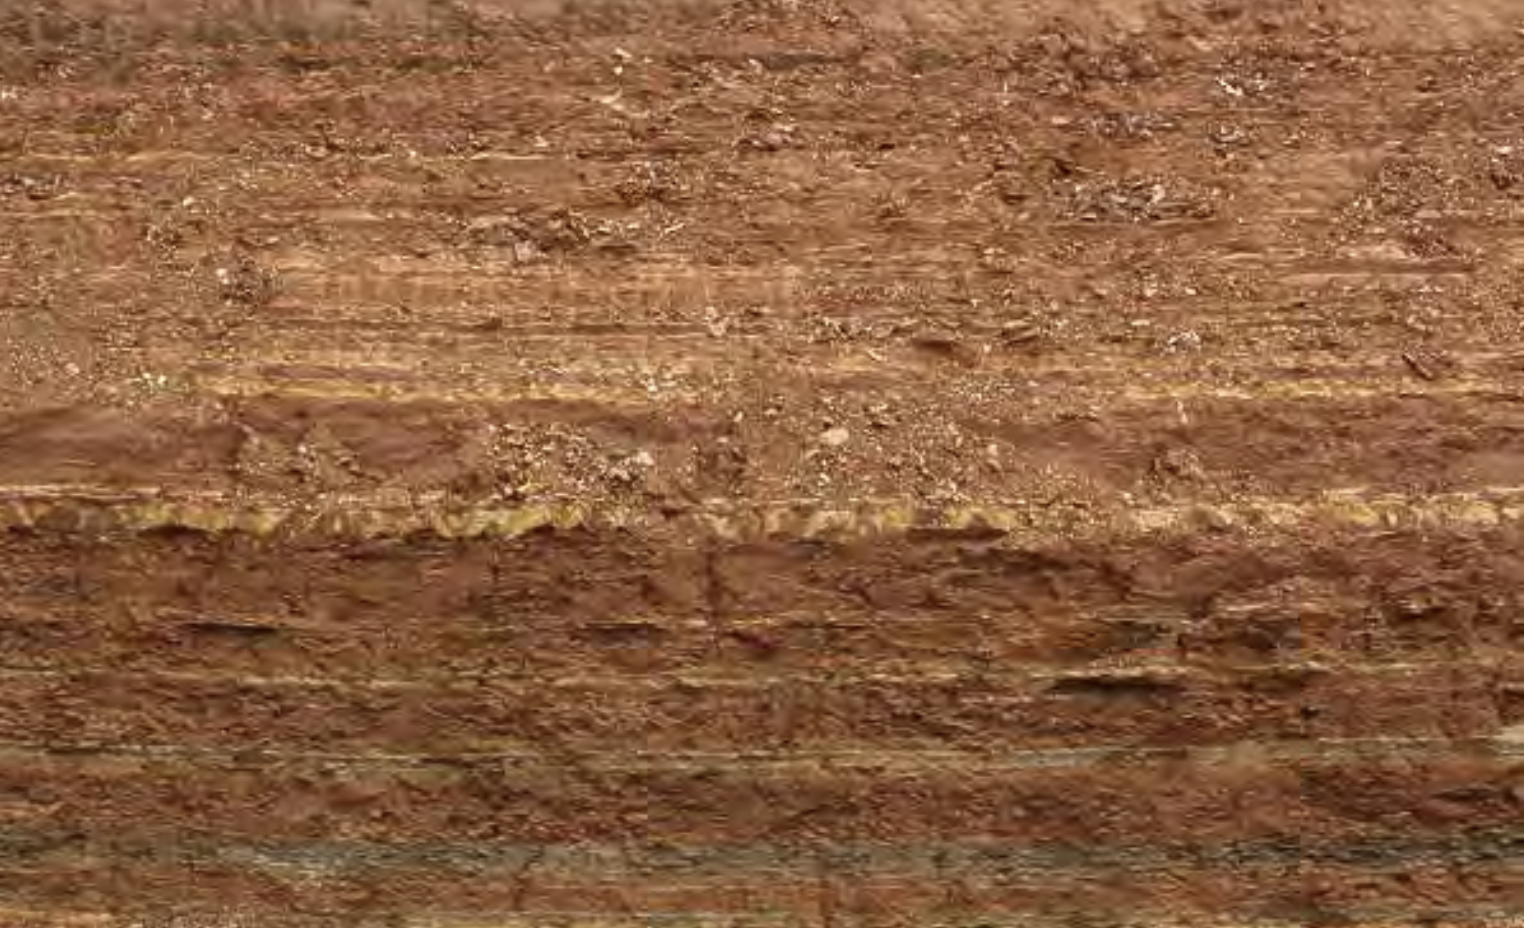
\includegraphics[width=0.8\textwidth]{layered-structure.png}
    \caption{Слоистая структура горной породы.}
\end{figure}

Обычно для математического моделирования ГРП целевой пласт представляется в виде слоистой среды, где каждый слой считается упругим изотропным сплошным телом, обладающим своими модулями упругости. Одной из используемых в практике является модель Planar3d ILSA \cite{DONTSOV201753}, используется для моделирования плоских магистральных трещин ГРП. Она основана на вариации метода граничных элементов --- методе разрывных смещений (МРС), \cite{dispalecement_discontinuty_Crouch1983}), в котором расчетная сетка строится только в плоскости трещины. Это позволяет уменьшить размерность матрицы упругости на единицу за счет сведения пространственной задачи к уравнениям на границе области с использованием аналитического решения уравнений упругости для однородной изотропной среды \cite{Peir2008}. Для слоистой среды не существует аналитического выражения для коэффициентов матрицы упругости, поэтому для обобщения данного метода использует следующие подходы.

Первый заключается в гомогенезации (осреднении) модулей упругости по всем слоям \cite{DONTSOV2021108144}. Преимуществом данного подхода является относительно простая реализация, за счет введения средних модулей упругости и сведения задачи к однородной изотропной среде. Однако данный подход не применим для слоистых структур с большой разницей упругих модулей и сред с включением тонких жестких пропластков.

Второй подход основан на численном построение матрицы упругости \cite{Siebrits_Peirce_2002,Peirce2001TheSF,Peirce2001UniformAA,Linkov1992}. Для этого применяют двумерное преобразование Фурье для определяющих уравнений упругой среды и далее, учитывая условия непрерывности компонент вектора смещений и нормальной нагрузки на границе раздела слоев, решают связанную задачу. После этого матрицу упругости восстанавливается путем применения обратного дискретного преобразования Фурье к полученному решению.

Целью данной работы является реализация метода построения численной матрицы упругости для слоистой среды с неоднородностью по модулям упругости и внедрение его в модель Planar3d ILSA, реализованной ранее в лаборатории цифровых и интеллектуальных систем добычи углеводородов в Институте гидродинамики им. М. А. Лаврентьева СО РАН. В работе проведен параметрический анализ задачи и показано существенное влияние неоднородности модулей упругости на геометрию трещины ГРП. Проведено сравнение влияния неоднородности сжимающих напряжений и модулей упругости слоев на геометрию финальной трещины ГРП. Изучено влияние тонких жестких пропластков на раскрытие трещины, что важно при расчете переноса расклинивающего агента (проппанта) и других компонент жидкости по трещине.


\clearpage    % Введение
\ifnumequal{\value{contnumfig}}{1}{\counterwithout{figure}{chapter}
}{\counterwithin{figure}{chapter}}
\ifnumequal{\value{contnumtab}}{1}{\counterwithout{table}{chapter}
}{\counterwithin{table}{chapter}}
\chapter{Постановка задачи}
\label{section:problem_formulation}

\begin{figure}[htbp]
    \centering
    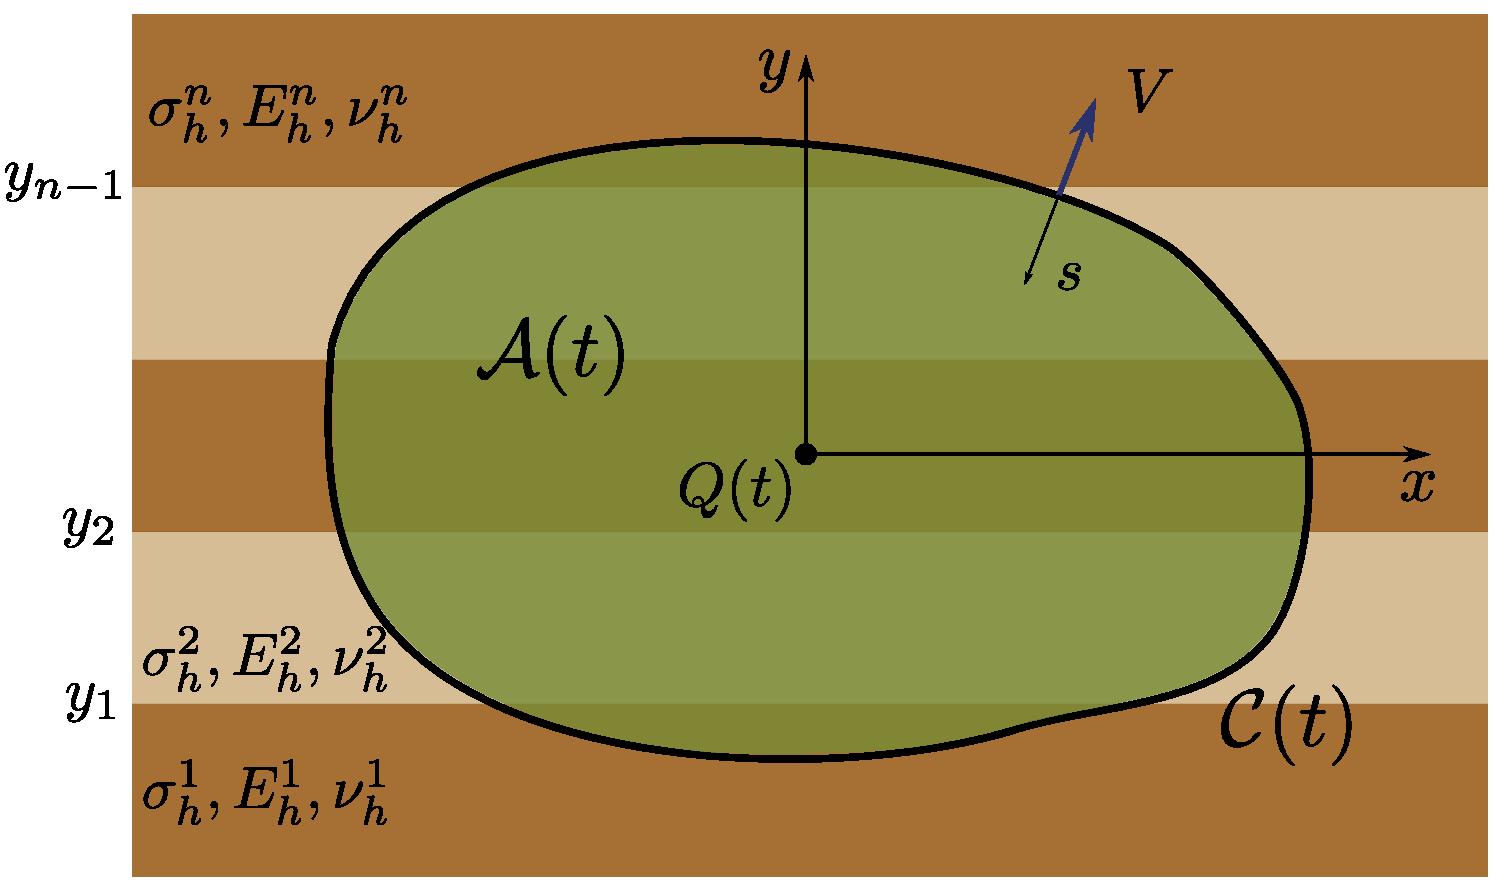
\includegraphics[width=0.7\textwidth]{fracture_scheme.pdf}
    \caption{Модель плоской трещины.}
    \label{fig:planar_fracture}
\end{figure}

Уравнение неразрывности в приближении тонкого слоя для плоской трещины (рисунок~\ref{fig:planar_fracture}) имеет вид
\begin{equation}
    \label{eq:conservation_law}
    \pd{w}{t} + \bigtriangledown \cdot q + \frac{2C_L}{\sqrt{t-t_0(x,\, y)}}  = Q(t) \delta(x,\,y),
\end{equation}
где $w(x,y,t)$ -- раскрытие трещины, $q(x,y,t)$ -- поток жидкости внутри трещины, $Q(t)$ -- объём закаченной в трещину жидкости. Утечки жидкости вычисляются согласно модели Картера~\cite{Cart1957}. $t_0(x,\, y)$ -- момент времени, в который фронт трещины находился в точке $(x, y)$.

Используя закон Пуазейля $q  = -\frac{w^3}{12\mu} \bigtriangledown\! p$ получим уравнение Рейнольдса \cite{DONTSOV201753}
\begin{equation}
    \label{eq:reynolds_equation}
    \pd{w}{t} - \text{div} \left( -\frac{w^3}{12\mu} \bigtriangledown \!p \right) + \frac{2C_L}{\sqrt{t-t_0(x,\, y)}}  = Q(t) \delta(x,\,y),
\end{equation}
где $\mu$ -- вязкость жидкости, $p(x,y,t)$ -- давление жидкости, действующее на поверхности трещины.

Уравнение упругости связывает раскрытие трещины $w$ с давлением $p$
\begin{equation}
    \label{eq:elasticity_equation}
    p(x,y,t) = \sigma_h(y) + \int\limits_{\mathcal{A}(t)} G(x,y;x',y')w(x',y',t) \dif x' \dif y',
\end{equation} 
где $\mathcal{A}(t)$ -- площадь плоской трещины, $\sigma_h$ -- сжимающие напряжение. В случае изотропной среды
\begin{equation}
    \label{eq:elasticity_kernel}
    G(x,y;x',y') = - \frac{E'}{8\pi [(x\!-\!x')^2+(y\!-\!y')^2]^{3/2}}.
\end{equation}
$E' = E / (1-\nu^2)$, где $E$ -- модуль Юнга, $\nu$ -- коэффициент Пуассона.

В случае неоднородности модулей упругости по слоям ядро $G(x,y;x',y')$ не имеет аналитический вид, и для его нахождения требуется численное построение.

Дискретизация уравнений \eqref{eq:reynolds_equation} и \eqref{eq:elasticity_equation} осуществляется с помощью МРС \cite{dispalecement_discontinuty_Crouch1983}. Для этого область разбивается на элементы $\mathcal{A}_{i,j}$ с помощью прямоугольной сетки. Центр ячейки $\mathcal{A}_{i,j}$ расположен в $(x_i,y_j)$ и имеет размеры $\Delta x$, $\Delta y$. Для раскрытия трещины $w$ и давления $p$ используется кусочно-постоянная аппроксимация
\begin{equation}
    \label{eq:piecewiece_approximation}
    \begin{split}
        w(x,y,t) &= \sum\limits_{i,j} w_{i,j}(t) H_{i,j}(x,y), \\
        p(x,y,t) &= \sum\limits_{i,j} p_{i,j}(t) H_{i,j}(x,y), \\
    \end{split}
\end{equation}
где 
\begin{equation}
    \label{eq:heaviside_function}
    H_{i,j}(x,y) = \left\{
        \begin{array}{ll}
            1, & (x,y) \in \mathcal{A}_{i,j}, \\
            0, & (x,y) \notin \mathcal{A}_{i,j}.
        \end{array}\right.
\end{equation}

Тогда уравнение упругости \eqref{eq:elasticity_equation} путём явного интегрирования по элементу сводится к
\begin{equation}
    \label{eq:discrete_elasticity}
    p_{i,j}(t) = {\sigma_h}_{i,j} + \sum\limits_{k,l} C_{i,j;k,l} w_{k,l}(t),
\end{equation}
где $C_{i,j;k,l}$ -- матрица упругости. Дискретизация уравнения Рейнольдса \eqref{eq:reynolds_equation} осуществляется путем интегрирования по времени и элементу \cite{DONTSOV201753}.           % Глава 1
\chapter{Матрица упругости для слоистой среды}
\label{sec:layered_elasticity}

В случае однородной изотропной среды коэффициенты матрицы упругости $C_{i,j;k,l}$ могут быть найдены аналитическим способом из \eqref{eq:elasticity_kernel} путем интегрирования ядра $G(x,y;x',y')$ на элементе $\mathcal{A}_{i,j}$ \cite{Peir2008}
\begin{equation}
    \label{eq:homogeneous_matrix}
    C_{i,j;k,l} = -\frac{E'}{8\pi} \left[\frac{\sqrt{(x_i\!-\!x)^2 + (y_j\!-\!y)^2}}{(x_i\!-\!x)(y_j\!-\!y)} \right]_{x=x_k-\Delta x/2, y=y_l-\Delta y/2}^{x=x_k+\Delta x/2, y=y_l+\Delta y/2},
\end{equation}
где $[f]_{x=x_1, y=y_1}^{x=x_2, y=y_2} = f(x_1,y_1) - f(x_1,y_2) - f(x_2,y_1) + f(x_2,y_2)$.

В случае неоднородности по модулям упругости слоистой среды требуется численное построение матрицы упругости. Будем считать, что каждый слой есть упругая изотропная среда. Определяющие уравнения упругой изотропной среды задаются формулами
\begin{equation}
    \label{eq:equilibrium}
    \sigma_{ij,j} + f_j = 0,
\end{equation}
\begin{equation}		
    \sigma_{ij} = \lambda e_{kk}\delta_{ij} + 2G e_{ij},
    \label{eq:hooke_law}
\end{equation}
где $\lambda = \frac{E \nu}{(1+\nu)(1-2\nu)}$ и $ G = \frac{E}{2(1+\nu)} $.

Отделяя производные по $y$ от производных по $x, z$ в (\ref{eq:equilibrium}) и (\ref{eq:hooke_law}) \cite{Siebrits_Peirce_2002,Peirce2001TheSF,Peirce2001UniformAA}, получим
\begin{equation}
    \label{eq:separate}
    \partial_{y} T = \mathbb{A}T + F,
\end{equation}
где
\begin{equation}
    \label{eq:T}
    \begin{split}
        T &= \left[\sigma_{yy} , \quad \sigma_{xy} , \quad \sigma_{yz} , \quad u_{y} , \quad u_{x} , \quad u_{z}\right]^T, \\
        F &= \left[-f_y , \quad -f_x , \quad -f_z , \quad 0 , \quad 0 , \quad 0\right]^T,
    \end{split}
\end{equation}

и $\mathbb{A}$ -- дифференциальный оператор, который содержит производные только по $x$ и $z$
\begin{equation}
    \label{eq:A}
    \mathbb{A} = 
    \left[\begin{array}{cccccc}
        0                      & -\partial_x & -\partial_z & 0 & 0 & 0 \\
        -\frac{b}{a}\partial_x & 0           & 0 & 0 & \frac{b^2-a^2}{a}\partial_{xx} - \frac{f}{2}\partial_{zz} & \left( \frac{b^2-ab}{a} - \frac{f}{2} \right) \partial_{xz} \\
        -\frac{b}{a}\partial_z & 0           & 0 & 0 & \left( \frac{b^2-ab}{a} - \frac{f}{2} \right) \partial_{xz} & \frac{b^2-a^2}{a}\partial_{zz} - \frac{f}{2}\partial_{xx} \\
        \frac{1}{a}            & 0           & 0 & 0 & -\frac{b}{a}\partial_x & -\frac{b}{a}\partial_z \\
        0                      & \frac{2}{f} & 0 & -\partial_x & 0 & 0 \\
        0                      & 0           & \frac{2}{f} & -\partial_z & 0 & 0 
    \end{array}\right],
\end{equation}

где используются константы
\begin{align*}
    a   & = \lambda + 2G,                          & b   & = \lambda,                &     f & = 2G, \\
    l_2 & = \frac{\lambda + 3G}{\lambda + G},      & l_4 & = \frac{2G^2}{\lambda+G}, &   l_5 & = \frac{2G(\lambda + 2G)}{\lambda + G}, \\
    l_6 & = \frac{2G(2\lambda + 2G)}{\lambda + G}, & l_7 & = \frac{2\lambda G}{\lambda+G}
\end{align*}


Применяя преобразование Фурье \eqref{eq:fourier_transform_2d} для системы \eqref{eq:separate} по координатам $x$ и $z$, получим
\begin{equation}
    \label{eq:FT_system}
    \partial_y \hat{T} = \hat{\mathbb{A}} \hat{T} + \hat{F},
\end{equation}
где
\begin{equation}
    \label{eq:FourierT}
    \begin{split}
        \hat{T} &= \left[\hat{\sigma}_{yy}/k , \quad \hat{\tau}_s/k , \quad \hat{u}_y , \quad \hat{u}_s , \quad  \hat{\tau}_t/k , \quad  \hat{u}_t \right]^T, \\
        \hat{F} &= \left[-\hat{f}_y , \quad -\hat{f}_s , \quad 0 , \quad 0 , \quad -\hat{f}_t , \quad 0\right]^T,
    \end{split}
\end{equation}
и оператор $\hat{\mathbb{A}}$
\begin{equation}
    \label{eq:FourierA}
    \hat{\mathbb{A}} = 
    \left[\begin{array}{cccccc}
        0 & -k & 0 & 0 & 0 & 0 \\
        \frac{b}{a}k & 0 & 0 & -\frac{b^2-a^2}{a}k^2 & 0 & 0 \\
        \frac{1}{a} & 0 & 0 & -\frac{b}{a}k & 0 & 0 \\
        0 & \frac{2}{f} & k & 0 & 0 & 0 \\
        0 & 0 & 0 & 0 & 0 & \frac{f}{2}k \\
        0 & 0 & 0 & 0 & \frac{2}{f} & 0 
    \end{array}\right].
\end{equation}

Здесь введены обозначения
\begin{equation}
    \label{eq:FT_special_variables}
    \begin{split}
        \hat{u}_s & = -i \frac{(m\hat{u}_x + n\hat{u}_z)}{k}, \\
        \hat{u}_t & = -i \frac{(n\hat{u}_x - m\hat{u}_z)}{k}, \\
        \hat{\tau}_s & = -i \frac{(m\hat{\sigma}_{xy} + n\hat{\sigma}_{yz})}{k}, \\
        \hat{\tau}_t & = -i \frac{(n\hat{\sigma}_{xy} - m\hat{\sigma}_{yz})}{k}. \\
    \end{split} 
\end{equation}

В случае $\hat{F} = 0$ система \eqref{eq:FT_system} является ОДУ и решение зависит от 6 свободных коэффициентов (\cite{Siebrits_Peirce_2002}, спектральные коэффициенты)
\begin{equation}
    \label{eq:fourier_solution}
    \left[
    \begin{array}{c}
        \hat{T}_s \\
        \hat{T}_t 
    \end{array}
    \right]
    =
    \left[
    \begin{array}{cc}
        Z_s & 0 \\
        0 & Z_t 
    \end{array}
    \right]
    \left[
    \begin{array}{c}
        A_s \\
        A_t 
    \end{array}
    \right]
\end{equation}

где используются обозначения
\begin{equation}
    \label{eq:FourierSeparateT}
    \hat{T}_s = \left[\hat{\sigma}_{yy}/k, \quad \hat{\tau}_s/k, \quad \hat{u}_y, \quad \hat{u}_s \right]^T, \qquad 
    \hat{T}_t = \left[ \hat{\tau}_t/k, \quad  \hat{u}_t \right]^T.
\end{equation}

Матрицы $Z_s$ и $Z_t$ имеют вид
\begin{equation}
    \label{eq:FourierSeparateA}
    \begin{split}
    Z_s & = 
    \left[
    \begin{array}{cccc}
        -fe^{-ky} & (l_4-fky)e^{-ky} & fe^{ky} & (l_4+fky)e^{ky} \\
        -fe^{-ky} & (l_5-fky)e^{-ky} & -fe^{ky} & -(l_5+fky)e^{ky} \\
        e^{-ky} & kye^{-ky} & e^{ky} & kye^{ky} \\
        e^{-ky} & (ky-l_2)e^{-ky} & -e^{ky} & -(ky+l_2)e^{ky} \\
    \end{array}
    \right],
    \\
    Z_t & = 
    \left[
    \begin{array}{cc}
        -\frac{f}{2}e^{-ky} & \frac{f}{2}e^{ky} \\
        e^{-ky} & e^{ky}
    \end{array}
    \right].
    \end{split}
\end{equation}

Из \eqref{eq:fourier_solution} получаем связь между спектральными коэффициентами и значениями смещений и напряжений на границе слоя
\begin{equation}
    \label{eq:As}
    \left[
    \begin{array}{c}
    A^{j}_{1}(k) \\
    A^{j}_{2}(k)\\
    A^{j}_{3}(k) \\
    A^{j}_{4}(k)
    \end{array}
    \right]
    = \frac{1}{2l^j_5}
    \left[
    \begin{array}{cccc}
        -l^j_2 & 0 & l^j_5 & -l^j_4 \\
        -1 & 1 & f^j & -f^j \\
        l^j_2 & 0 & l^j_5 & l^j_4 \\
        -1 & -1 & -f^j & -f^j
    \end{array}
    \right]
    \left[
    \begin{array}{c}
    \hat{\sigma}^{j}_{yy}(y=y_j)/k \\
    \hat{\tau}^{j}_{s}(y=y_j)/k\\
    \hat{u}^{j}_{y}(y=y_j) \\
    \hat{u}^{j}_{s}(y=y_j) 
    \end{array}
    \right],
\end{equation}

\begin{equation}
    \label{eq:At}
    \left[
    \begin{array}{c}
        A^{j}_{5}(k) \\
        A^{j}_{6}(k)
    \end{array}
    \right]
    = \frac{1}{2l^j_5}
    \left[
    \begin{array}{cc}
        -\frac{1}{f^j} & \frac{1}{2} \\
        \frac{1}{f^j} & \frac{1}{2}
    \end{array}
    \right]
    \left[
    \begin{array}{c}
    \hat{\tau}^{j}_{t}(y=y_j)/k\\
    \hat{u}^{j}_{t}(y=y_j) 
    \end{array}
    \right].
\end{equation}

\begin{figure}[htbp]
    \centering
    \begin{subfigure}[b]{0.45\textwidth}
        \centering
        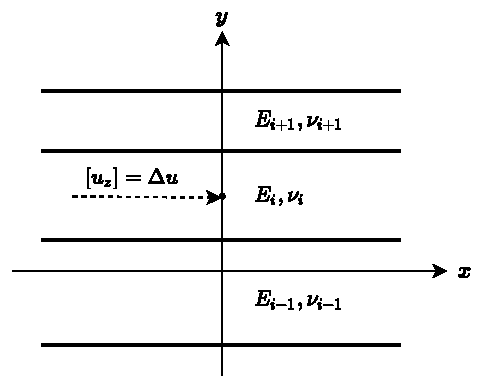
\includegraphics[width=\textwidth]{DD_point.pdf}
        \caption{Условие точечного разрыва смещений}
        \label{fig:DD_point}
    \end{subfigure}
    \hfill 
    \begin{subfigure}[b]{0.45\textwidth}
        \centering
        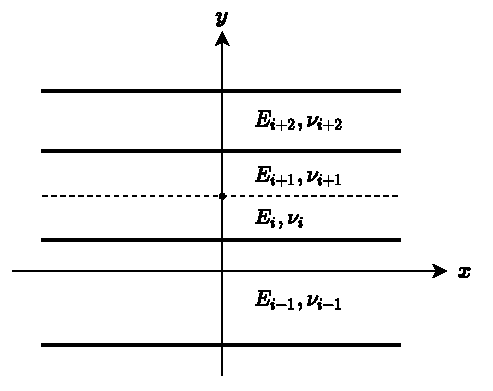
\includegraphics[width=\textwidth]{DD_point2.pdf}
        \caption{Введение дополнительной границы}
        \label{fig:pseudointerface}
    \end{subfigure}
    \caption{Введение псевдо-границы}
    \label{fig:Pseudointerface}
\end{figure}

Введём псевдо-границу (рисунок~\ref{fig:pseudointerface}) вдоль точки, в которой ставится условие разрыва смещений (рисунок~\ref{fig:DD_point}). Тогда $u_{z-0} - u_{z+0} = \Delta u$ может быть представлена в виде скачка смещения и напряжений на границе раздела слоев
\begin{multline}
    \label{eq:jump_condition}
    \left[ \hat{T} \right] = \hat{T}(y-0) - \hat{T}(y+0) = 
    \left[ \begin{array}{c} 
        0 \\ \frac{\Delta u(b^2 - a^2)}{a} \\ \frac{\Delta ub}{a} \\ 0 \\ 0 \\ 0 
    \end{array} \right]
    +
    \frac{m^2}{m^2+n^2} \left[ \begin{array}{c} 
        0 \\ \Delta u(a-b) \\ 0 \\ 0 \\ 0 \\ 0 
    \end{array} \right]
    + \\ +
    \frac{mn}{m^2+n^2} \left[ \begin{array}{c} 
        0 \\ 0 \\ 0 \\ 0 \\ \Delta u(a-b) \\ 0 
    \end{array} \right].
\end{multline}

Таким образом, мы получаем системы ОДУ для каждого слоя, связанные условиями неразрывности или \eqref{eq:jump_condition} на границе. Из этих соотношений можно составить уравнения для определения компонент вектора смещения и напряжений на границе раздела слоев
\begin{equation}
    \label{eq:coupled_t-system}
    A_t^i \hat{\tau}_t^{i-1} + C_t^i \hat{\tau}_t^{i} + B_t^i \hat{\tau}_t^{i+1} = D_t^i,
\end{equation}
для $t$-системы и 
\begin{equation}
    \label{eq:coupled_s-system}
    \textbf{A}_s^i \left[
        \begin{array}{c}
            \hat{\sigma}_{yy}^{i-1} \\
            \hat{\tau}_s^{i-1}
        \end{array}\right] +
    \textbf{C}_s^i \left[
        \begin{array}{c}
            \hat{\sigma}_{yy}^{i} \\
            \hat{\tau}_s^{i}
        \end{array}\right] + 
    \textbf{B}_s^i \left[
        \begin{array}{c}
            \hat{\sigma}_{yy}^{i+1} \\
            \hat{\tau}_s^{i+1}
        \end{array}\right]
    = \textbf{D}_s^i,
\end{equation}
для $s$-системы. Значения матриц в \eqref{eq:coupled_t-system} и \eqref{eq:coupled_s-system} приведены в Приложении~\ref{app:coupled_systems}.

Решая \eqref{eq:coupled_t-system} и \eqref{eq:coupled_s-system}, находим спектральные коэффициенты для каждого слоя из \eqref{eq:As} и \eqref{eq:At}. Окончательно, используя закон Гука \eqref{eq:hooke_law} и \eqref{eq:fourier_solution}, получим
\begin{multline}
    \label{eq:fourier_sigmazz}
    \hat{\sigma}^j_{zz}(y)/k = f\frac{n^2}{k^2}e^{-ky}A^j_1(k)
    - \left(l_6\frac{n^2}{k^2}+l_7\frac{m^2}{k^2}-f\frac{n^2}{k^2}ky \right)e^{-ky}A^j_2(k) - \\
    - f\frac{n^2}{k^2}e^{ky}A^j_3(k)
    - \left(l_6\frac{n^2}{k^2}+l_7\frac{m^2}{k^2}+f\frac{n^2}{k^2}ky \right)e^{ky}A^j_4(k) - \\
    - f\frac{mn}{k^2}e^{-ky}A^j_5(k)
    - f\frac{mn}{k^2}e^{ky}A^j_6(k).
\end{multline}
Применяя обратное дискретное преобразование Фурье \eqref{eq:DFT}, находим $\sigma_{zz}(y,x',y')$.

Условие \eqref{eq:jump_condition} является сингулярным в точке, в которой ставится условие разрыва смещений. Используя линейность определяющих уравнений \eqref{eq:equilibrium} и \eqref{eq:hooke_law}, можем представить ядро $G(x,y;x',y')$ для слоистой среды в виде
\begin{equation}
    G(x,y;x',y') = G_\text{hom}(x,y;x',y') + G'(x,y;x',y'),
\end{equation} 
где $G_\text{hom}(x,y;x',y')$ получается из \eqref{eq:elasticity_kernel} с учетом $E'=E'(y)$. Таким образом, удается избавится от сингулярности в условие \eqref{eq:jump_condition} и можем записать
\begin{equation}
    \label{eq:heterogeneous_kernel}
    G'(x,y;x',y') = -\Delta \sigma_{zz}(y, x', y'),
\end{equation}
где $\Delta \sigma_{zz}(y, x', y')$ находится из \eqref{eq:fourier_sigmazz}.
           % Глава 2
\chapter{Верификация и примеры расчетов}
\label{ch:verification}

Сравнение численного алгоритма, описанного выше, с МКЭ на задаче статического раскрытия трещины было показано в работе \cite{Peirce2001UniformAA}. В ней показана сопоставимость расчетов данных методов.

Чтобы продемонстрировать влияние неоднородности модулей упругости рассмотрим пласт, состоящий из трех слоев. Толщина внутреннего слоя $20$ м. Рассмотрим модель распространения трещины с равномерной закачкой жидкости в центре внутреннего слоя на протяжение всего процесса. Начальный момент времени $t = 0$~c., конечный $t = 300$~с., утечки жидкости в пласт отсутствуют. $E_i$, $\nu_i$, где $i=\text{b, m, t}$ -- упругие модули нижнего, среднего и верхнего слоев соответственно. 

В случае, если упругие модули всех слоев одинаковы получается модель радиальной трещины (рисунки \ref{fig:homogeneous-planar}, \ref{fig:homogeneous-slice}).
\begin{figure}[htbp]
    \centering
    \begin{subfigure}[t]{0.4\textwidth}
        \centering
        \caption{Раскрытие трещины.}
        \label{fig:homogeneous-planar}
        \includegraphics[width=\textwidth]{Homogeneous/Figures/1/width_29.pdf}
    \end{subfigure}
    \hfill 
    \begin{subfigure}[t]{0.55\textwidth}
        \centering
        \caption{Раскрытие трещины вдоль оси $Oy$, $x=1.5$~м.}
        \label{fig:homogeneous-slice}
        \includegraphics[width=\textwidth]{Homogeneous/Figures/1/w_y_29.pdf}
    \end{subfigure}
    \caption{Радиальная трещина, $E_\text{b} = E_\text{m} = E_\text{t} = 10$~GPa, $\nu_\text{b} = \nu_\text{m} = \nu_\text{t} = 0.22$.}
    \label{fig:homogeneous}
\end{figure}

Рассмотрим пласт, где модуль Юнга $E_\text{b}$ нижнего слоя выше, чем в верхних. Как видно из рисунков~\ref{fig:heterogeneous-2-layer-planar} и \ref{fig:heterogeneous-2-layer-slice} жесткость нижнего слоя сильно влияет на распространение трещины. Расстояние от верхнего кончика трещины до точки закачки жидкости ГРП больше в два раза, чем расстояние от нижнего кончика трещины.
\begin{figure}[htbp]
    \centering
    \begin{subfigure}[t]{0.4\textwidth}
        \centering
        \caption{Раскрытие трещины.}
        \label{fig:heterogeneous-2-layer-planar}
        \includegraphics[width=\textwidth]{Heterogeneous/Figures/1/width_29.pdf}
    \end{subfigure}
    \hfill 
    \begin{subfigure}[t]{0.55\textwidth}
        \centering
        \caption{Раскрытие трещины вдоль оси $Oy$, $x=1.5$~м.}
        \label{fig:heterogeneous-2-layer-slice}
        \includegraphics[width=\textwidth]{Heterogeneous/Figures/1/w_y_29.pdf}
    \end{subfigure}
    \caption{Пласт с жестким нижним слоем, $E_\text{b} = 50$~GPa, $E_\text{m} = E_\text{t} = 10$~GPa, $\nu_\text{b} = \nu_\text{m} = \nu_\text{t} = 0.22$.}
    \label{fig:heterogeneous-2-layer}
\end{figure}


Стоит заметить, что в отличие от неоднородности по сжимающим напряжениям, неоднородность по модулям упругости не образует барьер для роста трещины. Даже при большой разницы модулей Юнга трещина проникает и растет вдоль жесткого слоя. На рисунке~\ref{fig:heterogeneous-high} показан результат для $k=\frac{E_\text{b}}{E_\text{t}} = 10$. На рисунке~\ref{fig:heterogeneous-3layer} изображен случай, где средний слой ограничен более жесткими. Подобный результат был также показан на модели Pseudo3d в работе~\cite{gu2006}.
\begin{figure}[htbp]
    \centering
    \begin{subfigure}[t]{0.4\textwidth}
        \centering
        \caption{Раскрытие трещины.}
        \label{fig:heterogeneous-high-planar}
        \includegraphics[width=\textwidth]{Heterogeneous/Figures/2/width_29.pdf}
    \end{subfigure}
    \hfill 
    \begin{subfigure}[t]{0.55\textwidth}
        \centering
        \caption{Раскрытие трещины вдоль оси $Oy$, $x=1.5$~м.}
        \label{fig:heterogeneous-high-slice}
        \includegraphics[width=\textwidth]{Heterogeneous/Figures/2/w_y_29.pdf}
    \end{subfigure}
    \caption{Пласт с сильной неоднородностью, $E_\text{b} = 100$~GPa, $E_\text{m} = E_\text{t} = 10$~GPa, $\nu_\text{b} = \nu_\text{m} = \nu_\text{t} = 0.22$.}
    \label{fig:heterogeneous-high}
\end{figure}


\begin{figure}[htbp]
    \centering
    \begin{subfigure}[t]{0.4\textwidth}
        \centering
        \caption{Раскрытие трещины.}
        \label{fig:heterogeneous-3layer-planar}
        \includegraphics[width=\textwidth]{Heterogeneous/Figures/3_3/width_29.pdf}
    \end{subfigure}
    \hfill 
    \begin{subfigure}[t]{0.55\textwidth}
        \centering
        \caption{Раскрытие трещины вдоль оси $Oy$, $x=1.5$~м.}
        \label{fig:heterogeneous-3layer-slice}
        \includegraphics[width=\textwidth]{Heterogeneous/Figures/3_3/w_y_29.pdf}
    \end{subfigure}
    \caption{Пласт с сильной неоднородностью, $E_\text{m} = 10$~GPa, $E_\text{b} = E_\text{t} = 100$~GPa, $\nu_\text{b} = \nu_\text{m} = \nu_\text{t} = 0.22$.}
    \label{fig:heterogeneous-3layer}
\end{figure}


Рассмотрим случай, где также присутствует неоднородность сжимающих напряжений. В верхних слоях $\sigma_{h,\text{m}} = \sigma_{h,\text{t}} = 30.5$~MPa выше, чем в нижнем $\sigma_{h,\text{b}} = 30$~MPa. Из рисунка~\ref{fig:comparison-1} видно, что рост трещины обусловлен ростом в нижнем слое, несмотря на то, что его модуль Юнга $E_\text{b} = 20$~GPa больше, чем в верхних слоях $E_\text{m} = E_\text{t} = 10$~GPa. Подобное поведение роста трещины связано с тем, что эффективное напряжение $p_\text{net} = p - \sigma_h$ -- выше в нижнем слое. На рисунке~\ref{fig:comparison-2} приведен пример, где модуль Юнга $E_\text{b} = 40$~GPa компенсирует высокое эффективное напряжение.

\begin{figure}[htbp]
    \centering
    \begin{subfigure}[t]{0.4\textwidth}
        \centering
        \caption{Раскрытие трещины.}
        \label{fig:comparison-1-planar}
        \includegraphics[width=\textwidth]{Heterogeneous/Figures/3/width_29.pdf}
    \end{subfigure}
    \hfill 
    \begin{subfigure}[t]{0.55\textwidth}
        \centering
        \caption{Раскрытие трещины вдоль оси $Oy$, $x=1.5$~м.}
        \label{fig:comparison-1-slice}
        \includegraphics[width=\textwidth]{Heterogeneous/Figures/3/w_y_29.pdf}
    \end{subfigure}
    \caption{Неоднородный по модулям упругости и сжимающим напряжениям пласт, $E_\text{b} = 20$~GPa, $E_\text{m} = E_\text{t} = 10$~GPa, $\nu_\text{b} = \nu_\text{m} = \nu_\text{t} = 0.22$, $\sigma_{h,\text{b}} = 30$~MPa, $\sigma_{h,\text{m}} = \sigma_{h,\text{t}} = 30.5$~MPa,.}
    \label{fig:comparison-1}
\end{figure}


\begin{figure}[htbp]
    \centering
    \begin{subfigure}[t]{0.4\textwidth}
        \centering
        \caption{Раскрытие трещины.}
        \label{fig:comparison-2-planar}
        \includegraphics[width=\textwidth]{Heterogeneous/Figures/3_2/width_29.pdf}
    \end{subfigure}
    \hfill 
    \begin{subfigure}[t]{0.55\textwidth}
        \centering
        \caption{Раскрытие трещины вдоль оси $Oy$, $x=1.5$~м.}
        \label{fig:comparison-2-slice}
        \includegraphics[width=\textwidth]{Heterogeneous/Figures/3_2/w_y_29.pdf}
    \end{subfigure}
    \caption{Неоднородный по модулям упругости и сжимающим напряжениям пласт, $E_\text{b} = 40$~GPa, $E_\text{m} = E_\text{t} = 10$~GPa, $\nu_\text{b} = \nu_\text{m} = \nu_\text{t} = 0.22$, $\sigma_{h,\text{b}} = 30$~MPa, $\sigma_{h,\text{m}} = \sigma_{h,\text{t}} = 30.5$~MPa,.}
    \label{fig:comparison-2}
\end{figure}


Рассмотрим пласт с включением тонкого жесткого слоя (толщина слоя $d$ меньше $10\%$ от диаметра трещины). Как видно из рисунков~\ref{fig:thin-layer-1} и \ref{fig:thin-layer-2} тонкие пропластки не ограничивают рост трещины. Однако раскрытие трещины в них ниже, чем в прилегающих слоях. Это может существенно сказаться на распространение проппанта. 
\begin{figure}[htbp]
    \centering
    \begin{subfigure}[t]{0.4\textwidth}
        \centering
        \caption{Раскрытие трещины.}
        \includegraphics[width=\textwidth]{Heterogeneous/Figures/4/width_29.pdf}
    \end{subfigure}
    \hfill 
    \begin{subfigure}[t]{0.55\textwidth}
        \centering
        \caption{Раскрытие трещины вдоль оси $Oy$, $x=1.5$~м.}
        \includegraphics[width=\textwidth]{Heterogeneous/Figures/4/w_y_29.pdf}
    \end{subfigure}
    \caption{Пласт с включением тонкого слоя, $d=10$~м. , $k=\frac{E_d}{E}=5$.}
    \label{fig:thin-layer-1}
\end{figure}

\begin{figure}[htbp]
    \centering
    \begin{subfigure}[t]{0.4\textwidth}
        \centering
        \caption{Раскрытие трещины.}
        \includegraphics[width=\textwidth]{Heterogeneous/Figures/5/width_29.pdf}
    \end{subfigure}
    \hfill 
    \begin{subfigure}[t]{0.55\textwidth}
        \centering
        \caption{Раскрытие трещины вдоль оси $Oy$, $x=1.5$~м.}
        \includegraphics[width=\textwidth]{Heterogeneous/Figures/5/w_y_29.pdf}
    \end{subfigure}
    \caption{Пласт с включением двух тонких пропластков, $d=10$~м. , $k=\frac{E_d}{E}=5$.}
    \label{fig:thin-layer-2}
\end{figure}           % Глава 3
\chapter*{Заключение}                       % Заголовок
\addcontentsline{toc}{chapter}{Заключение}
\label{sec:conclusion} 

\textbf{Основные результаты работы} заключаются в следующем:
\begin{enumerate}
    \item Реализован алгоритм построения численной матрицы упругости для метода разрывных смещений в случае неоднородных по модулю упругости слоев на языке программирования~C++.
    \item Выполнено встраивание данного алгоритма в модель раскрытия трещины гидроразрыва пласта Planar3d ILSA.
    \item Проведена верификация метода путем сравнения с известными литературными данными и точными решениями.
    \item Проведен анализ влияния учета слоистой структуры пласта на конечную геометрию трещины.
    \item Показано, что тонкие жесткие пропластки не существенно ограничивают рост трещины в вертикальном направлении, однако влияют на раскрытие трещины в них, что может сильно сказаться на распространение проппанта и конечной геометрии трещины ГРП. 
\end{enumerate}      % Заключение
% \include{Dissertation/acronyms}        % Список сокращений и условных обозначений
% \include{Dissertation/dictionary}      % Словарь терминов
\include{Dissertation/references}      % Список литературы
\clearpage
\ifdefmacro{\microtypesetup}{\microtypesetup{protrusion=false}}{} % не рекомендуется применять пакет микротипографики к автоматически генерируемым спискам
\listoffigures  % Список изображений

% %%% Список таблиц %%%
% % (ГОСТ Р 7.0.11-2011, 5.3.10)
% \clearpage
% \listoftables   % Список таблиц
% \ifdefmacro{\microtypesetup}{\microtypesetup{protrusion=true}}{}
% \newpage           % Списки таблиц и изображений (иллюстративный материал)

\setcounter{totalchapter}{\value{chapter}} % Подсчёт количества глав

%%% Настройки для приложений
\appendix
% Оформление заголовков приложений ближе к ГОСТ:
\setlength{\midchapskip}{20pt}
\renewcommand*{\afterchapternum}{\par\nobreak\vskip \midchapskip}
\renewcommand\thechapter{\Asbuk{chapter}} % Чтобы приложения русскими буквами нумеровались

\chapter{Дискретизация уравнения Рейнольдса}
\label{app:discrete-reynolds}

Интегрируя уравнение Рейнольдса~\eqref{eq:reynolds_equation} по времени от $t-\Delta t$ до $t$, где $\Delta t$ --- шаг по времени, и элементу $\mathcal{A}_{i,j}$, получим дискретизацию по методу конечных объемов
\begin{equation}
    \label{eq:discrete-reynolds}
    w_{i, j}(t) - w_{i, j}(t-\Delta t) = \Delta t[Ap]_{i, j} + \Delta t Q_{i, j} - \Delta \mathcal{L}_{i, j},
\end{equation}
где $\Delta t Q_{i, j}$ отвечает за закачку, $\Delta \mathcal{L}_{i, j}$ --- утечка жидкости в пласт с момента времени $t-\Delta t$ до $t$. $[Ap]_{i, j}$ --- это потоки жидкости через границу элемента $\mathcal{A}_{i,j}$, которые вычисляются как

\begin{equation}
    \begin{split}
        [Ap]_{i, j} &= \frac{1}{\Delta x} \left[M_{i+\frac{1}{2},j} \frac{p_{i+1,j}-p_{i,j}}{\Delta x} + M_{i-\frac{1}{2},j} \frac{p_{i-1,j}-p_{i,j}}{\Delta x} \right] + \\
        &= \frac{1}{\Delta y} \left[M_{i,j+\frac{1}{2}} \frac{p_{i,j+1}-p_{i,j}}{\Delta y} + M_{i,j+\frac{1}{2}} \frac{p_{i-1,j}-p_{i,j}}{\Delta y} \right],
    \end{split}
\end{equation}
где соответствующие мобильности жидкости определяются как
\begin{equation}
    M_{i \pm \frac{1}{2},j} = \frac{w^3_{i \pm 1,j} + w^3_{i,j}}{2\mu'}.
\end{equation}

Задача численного моделирования раскрытия трещины ГРП состоит в решении системы уравнений \eqref{eq:discrete-reynolds} и \eqref{eq:discrete_elasticity}.

\chapter{Связанные t- и s- системы}
\label{app:coupled_systems}

\section*{Решение t-системы}

Коэффициенты в t-системе \eqref{eq:coupled_t-system} имеют вид
\begin{equation}
    \label{eq:coefficients_t-system}
    \begin{split}
        A^{i}_t &= \frac{2}{f^{i}}\text{cosech}(kd^{i}),\\
        B^{i}_t &= \frac{2}{f^{i+1}}\text{cosech}(kd^{i+1}),\\
        C^{i}_t &= -\frac{2}{f^{i+1}}\coth(kd^{i+1}) - \frac{2}{f^{i}}\coth(kd^{i}),\\
        D^{i}_t &= \Delta \hat{u}^{i}_{t} + \frac{2}{f^{i+1}}\coth(kd^{i+1})\Delta\hat{\tau}_{t}^{i} 
        - \frac{2}{f^{i}}\text{cosech}(kd^{i})\Delta\hat{\tau}_{t}^{i-1},
    \end{split}
\end{equation}
где $d^i$ -- толщина $i$-го слоя, $\Delta \hat{u}^{i}_{t}$ и $\Delta\hat{\tau}_{t}^{i}$ значения скачков через границы слоев, связанных с введением дополнительной границы \eqref{eq:jump_condition}.

Смещение $\hat{u}^{i}_{t}$ на верхней границе $i$-го слоя можно найти, как
\begin{equation}
    \label{eq:upper_displacement_t}
    \hat{u}^{i}_{t} = \frac{2}{f^{i}}\coth(kd^{i})\hat{\tau}^{i}_{t} - \frac{2}{f^{i}}\text{cosech}(kd^{i}) (\hat{\tau}^{i-1}_{t} + \Delta\hat{\tau}^{i-1}_{t}).
\end{equation}
Находя $\hat\tau_t^i$ из \eqref{eq:coupled_t-system} и $\hat{u}^i_t$ из \eqref{eq:upper_displacement_t}, получаем вектор $\hat T_t^i$.


\section*{Решение s-системы}

Матрицы в s-системе \eqref{eq:coupled_s-system} задаются как
\begin{equation}
    \label{eq:coefficients_s-system}
    \begin{split}
        \textbf{A}^{i} & = -R^{i}_{tb},\\
        \textbf{C}^{i} & = R^{i+1}_{bb}-R^{i}_{tt},\\
        \textbf{B}^{i} & = R^{i+1}_{bt},\\
        \textbf{D}^{i} & = \Delta u^{i}-R^{i+1}_{bb}\Delta p^{i}+R^{i}_{tb}\Delta p^{i-1},
    \end{split}
\end{equation}
где используются следующие соотношения:
\begin{equation}
    \label{eq:R_matrix}
    \begin{split}
        p^i & = \left[\begin{array}{c}
            \hat{\sigma}_{yy}^{i} \\
            \hat{\tau}_s^{i}
        \end{array}\right],\\
        R_{tt} & = \frac{1}{D} \left[\begin{array}{cc}
            - l_{5}(th + k \cdot d \cdot se^{2}) & - (l_{4}\cdot th^{2} + f\cdot k^{2} \cdot d^{2} \cdot se^{2})\\
            - (l_{4}\cdot th^{2} + f\cdot k^{2} \cdot d^{2} \cdot se^{2})  & - l_{5}(th - k \cdot d \cdot se^{2}) 
        \end{array}\right],\\
        R_{bb} & = \frac{1}{D} \left[\begin{array}{cc}
            l_{5}(th + k \cdot d \cdot se^{2}) & - (l_{4}\cdot th^{2} + f\cdot k^{2} \cdot d^{2} \cdot se^{2}) \\
            - (l_{4}\cdot th^{2} + f\cdot k^{2} \cdot d^{2} \cdot se^{2})  & l_{5}(th - k \cdot d \cdot se^{2})
        \end{array}\right],\\
        R_{bt} & = \frac{1}{D} \left[\begin{array}{cc}
            - (th + k \cdot d)\cdot se & - k \cdot d \cdot th \cdot se \\
            k \cdot d \cdot th \cdot se & - (th - k \cdot d)\cdot se 
        \end{array}\right],\\
        R_{tb} & = \frac{1}{D} \left[\begin{array}{cc}
            (th + k \cdot d)\cdot se & - k \cdot d \cdot th \cdot se \\
            k \cdot d \cdot th \cdot se & (th - k \cdot d)\cdot se  
        \end{array}\right].\\
    \end{split}
\end{equation}
Для удобства используем следующие обозначения: $th = \tanh(kd)$, $se = \text{sech}(kd)$ и $D = f^{2}[(1 \!+\! k^{2} d^{2}) se^{2} \!-\! 1]$, где $d$ -- толщина слоя.

Смещения $\hat{u}^{i}_{y}$ и $\hat{u}^{i}_{s}$ на верхней границе $i$-го слоя можно найти, как
\begin{equation}
    \begin{bmatrix}
        \hat{u}^{i}_{y} \\
        \hat{u}^{i}_{s}
    \end{bmatrix}
    =
    R_{tt}^{i}
    \begin{bmatrix}
        \hat{\sigma}^{i}_{yy} \\
        \hat{\tau}^{i}_{s}
    \end{bmatrix}
    +
    R_{tb}^{i}
    \begin{bmatrix}
        \hat{\sigma}^{i-1}_{yy} + \Delta\hat{\sigma}^{i-1}_{yy} \\
        \hat{\tau}^{i-1}_{s} + \Delta\hat{\tau}^{i-1}_{s}
    \end{bmatrix}.
\end{equation}

\chapter{Fourier transform}
\label{ch:fourier_transform}

В работе используется следующее двумерное преобразование Фурье:
\begin{equation}
    \label{eq:fourier_transform_2d}
    \hat{f}(m,n) = \int\limits_{-\infty}^{\infty}  \int\limits_{-\infty}^{\infty} f(x,z) e^{-i(mx+nz)} \dif x \dif z,
\end{equation}
и обратное преобразование Фурье
\begin{equation}
    \label{eq:inverse_fourier_transform_2d}
    f(x,y) = \frac{1}{(2\pi)^2}\int\limits_{-\infty}^{\infty}  \int\limits_{-\infty}^{\infty} \hat{f}(m,n) e^{i(mx+nz)} \dif m \dif n
\end{equation}

Для численного построения матрицы упругости используем дискретное преобразование Фурье
\begin{align}
    \label{eq:DFT}
    \hat{f}(m, n) &= \sum_{i=0}^{N_x-1}\sum_{j=0}^{N_y-1} f(i,j)e^{-2\pi i \left(\frac{mi}{N_x}+\frac{nj}{N_y} \right)} \\
    f(i,j) &= \frac{1}{N_x N_y} \sum_{m=0}^{N_x-1}\sum_{n=0}^{N_y-1} \hat{f}(m, n)e^{2\pi i \left(\frac{mi}{N_x}+\frac{nj}{N_y} \right)}
\end{align}

\setcounter{totalappendix}{\value{chapter}} % Подсчёт количества приложений

\end{document}
